	%Linea Para poder completar automaticamente las citas con el Sublime
%No hace el documento, se puede borrar esta linea si no se usa el Sublime
%------------------------------------------------------------------------------
 \newcommand{\NoBiblioEQ}[1]{
 \ifthenelse{\equal{#1}{verdadero}}{}{\bibliography{Referencias/base_bibliografica}}
 \NoBiblioEQ{verdadero}}
 %----------------------------------------------------------------------------- 

%Formato (Nombre de capitulo largo o corto), nombre del capitulo y estilo de la
%Portada del Capitulo
%------------------------------------------------------------------------------

 %Formato en si, titulo en un solo renglon
 \FormatoCapituloDosLineas
 
 %Nombre y etiquete para referir
 \chapter{Electroquímica en películas delgadas mesoporosas}
 \label{chap:Electroquimica}

 %Para que no salga el numero de pagina en la portada del capitulo
 \thispagestyle{empty}
	
 %Resumen del Capitulo en Italica
 %\noindent\textit{En este capítulo se estudian exhaustivamente los fenómenos de transporte de sondas a través de las películas delgadas mesoporosas y su respuesta electroquímica. Analizando los resultados obtenidos por voltametría cíclica, voltametría cíclica de corriente alterna y simulaciones por elementos finitos. Se sugiere un modelo de transporte para cada caso y se calculan parámetros para los distintos sistemas, como concentración dentro las poros, coeficiente de difusión, constante de Langmuir y estabilidad química, entre otros.}

 %Indice de capitulo alineada al borde inferior de la pagina, nueva pagina
 \vfill
 \minitoc
 \newpage
 %-------------------------------------------------------------------------------

\section{Introducción}

	Luego de obtener y analizar los resultados de depositar, condensar y extraer \pdm\space sobre distintos sustratos y bajo diferentes tratamientos pos-depósito, se dedicará este capítulo al estudio de las propiedades de los sensores para detectar y cuantificar una variedad de sondas electroquímicas. Estas sondas, dadas sus cualidades, permitirán obtener información acerca del transporte a través de los sistemas nanoporosos. Los sensores están compuestos básicamente de una película delgada de oro sobre la cual se deposita  una película delgada mesoporosa de sílice. La superficie de las paredes dejan expuestos, hacia el interior de los poros, grupos silanoles los cuales pueden estar o no protonados.\cite{Brinker1990,Soler-Illia2011} 
			\begin{equation}
				\begin{aligned}
				\includegraphics[scale=0.75]{Esquemas/equilibriosilica.pdf}
				\label{eq:equilibriosilica}
				\end{aligned}
				\end{equation}
	Las reacciones \ref{eq:equilibriosilica} ejemplifican el equilibrio ácido-base que se establece en la superficie de una película de sílice. El pK$_{a2}$ del $\text{SiO}_2$ es menor a 4 y la mayoría de los autores coinciden en que el punto isoeléctrico (IEP) varía de $1$ a $4$ dependiendo de  las distintas formas morfológicas del óxido de silicio, en particular para el SiO$_2$ sintetizado vía sol-gel el $\text{IEP}\approx 2$ \cite{Kosmulski2002,Kosmulski2014,Schwarz1984,Si-HanWu2013}.
	Wu y colaboradores\cite{Si-HanWu2013} analizaron, por un lado, el estado de carga superficial de nanopartículas de sílice mesoporosa y, por otro, la velocidad de condensación. El gráfico de la figura \ref{fig:silica_ph} muestra como varían las razones  $\text{SiO}^{-}/\text{SiOH}$ y $\text{SiOH}_2^{+}/\text{SiOH}$ en función del pH; se puede apreciar que solo por encima de $\text{pH}\geq7$ se obtiene una superficie de carga negativa donde todos los silanoles reaccionaron, cediendo su $\text{H}^{+}$, para convertirse en iones silanoatos; mientras que para pH bajos ($\text{pH}\leq1$), la sílice se vuelve inestable antes de llegar a un estado de carga completamente positivo y, solo queda, parcialmente positiva. 
		\begin{figure}[bh!]
			\begin{subfigure}[t]{0.73\textwidth}
 	       	\includegraphics[width=\textwidth]{Graficos/Silica-PH-Stability.jpg}
 	       	\end{subfigure}
 	       	\begin{subfigure}[t]{0.25\textwidth}
 	       	 	\includegraphics[scale=0.80]{Esquemas/carga-PI.pdf}
	      	 \end{subfigure}
	    	\caption[Velocidad de condensación y estado de carga superficial]{Velocidad de condensación y estado de carga superficial para nanoparticulas de sílice en función de pH. Gráfico extraído de \textit{Synthesis of mesoporous silica nanoparticles} Chem. Soc. Rev., 42(9):3862, 2013.\cite{Si-HanWu2013}}
	       	\label{fig:silica_ph}
	    	\end{figure}
	En el mismo trabajo\cite{Si-HanWu2013} también plantean que la velocidad de condensación decrece por encima de $\text{pH}\geq7.5$ debido a que entra en una zona de inestabilidad donde el óxido se disuelve, catalizado por el medio básico.
	    	
	De hecho, Iler, en su libro \textit{<<The Chemistry of Silica>>}, explica que la velocidad de disolución de la sílice en medio acuoso depende de muchos factores y, que además, dependiendo el tipo de sílice, el proceso de disolución requiere de un catalizador. Presenta un gráfico de la velocidad de disolución en función del pH (figura \ref{fig:disolucion_ph}) y postula que la misma depende de la forma que adopte la sílice, ya sea cristalina o amorfa. Para formas menos organizadas, como el SiO$_2$ amorfo, la cinética de disolución es más rápida, mientras que para otras, más cristalinas, como el cuarzo, se hace mucho mas lenta. Por último aclara que se trata de un proceso de despolimerización vía hidrólisis, y que la solubilidad es la concentración de Si(OH)$_4$ cuando alcanza un estado estacionario en el equilibrio despolimerazación-polimerización.\cite{iler1979,blesa1994}. 

			\begin{figure}[th!]
			    \begin{center}
			    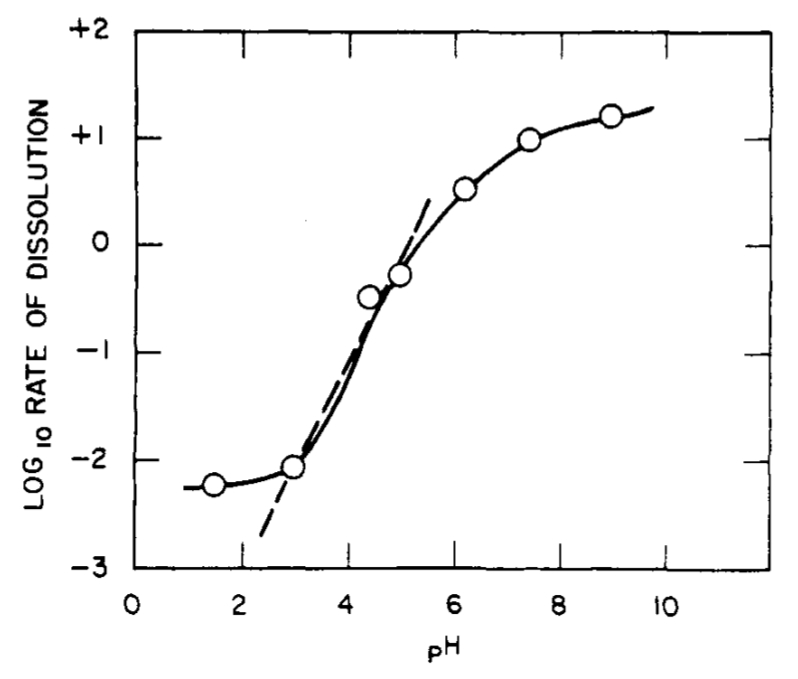
\includegraphics[width=0.70\textwidth]{Graficos/disolucion_ph.jpg}
	       		\caption[Velocidad de disolución sílice en función del pH]{Velocidad de disolución de la sílice en función de pH. Gráfico extraído de \textit{The chemistry of silica} Wiley 1ª edición, 1979.\cite{iler1979}}
	         	\label{fig:disolucion_ph}
	     		\end{center}
	     		\end{figure}
	
	También propone un mecanismo en medio ácido catalizado por iones F$^-$, mientras que en medio básico el mecanismo es catalizado por iones OH$^-$, según el siguiente mecanismo:
		
			\begin{equation}
				\begin{aligned}
				\includegraphics[scale=0.63]{Esquemas/disolucion-silica.pdf}
				\label{eq:disolucionsilica}
				\end{aligned}
				\end{equation} 
	
	El mecanismo de \ref{eq:disolucionsilica} no está completamente consensuado en la literatura especializada. Sin embargo, todos los autores coinciden en que el óxido se vuelve inestable en cualquiera de sus formas a partir de un $\text{pH}\geq7$ y que, a partir de $\text{pH}\geq10$ el proceso de disolución se acelera varios ordenes de magnitud.\cite{Kosmulski2002,Kosmulski2014,Schwarz1984,Si-HanWu2013,iler1979} En 2007 Bass y colaboradores\cite{bass2007} realizaron un estudio completo sobre la estabilidad de películas de óxidos mesoporososos de SiO$_2$, Zr$_X$Si$_{1-X}$O$_2$, Al$_X$Si$_{1-X}$O$_2$ y TiO$_2$ en condiciones fisiológicas (pH$=7.4$), llegando a la conclusión de que la sílice mesoporosa se disuelve rápidamente mientras que es más estable con un pequeño agregado de circonio o aluminio en su estructura.

	%Este capitulo tiene por objetivo comprender los fenómenos de transporte dentro de las películas mesoporososas mediante técnicas electroquímicas. 

	Son muchos los trabajos que aplican técnicas de electroquímica a electrodos recubiertos con \pdm\space (de distintos óxidos, funcionalizados y sin funcionalizar), ya sea para caracterizar el material o para potenciales aplicaciones. Se pueden citar ejemplos que utilizan EQ como herramientas para evaluar la accesibilidad de las películas en función de la organización espacial de los poros\cite{Etienne2007,Herzog2013}, caracterizar el área especifica libre del electrodo \cite{Otal2006} o caracterizar el transporte de masa dentro de los poros\cite{Calvo2009,brunsen2011}. Dentro de los trabajos que sugieren aplicaciones, podemos encontrar aquellos que los usan como membranas permeoselectiva \cite{Fattakhova-Rohlfing2007,Andrieu-Brunsen2015,Calvo2009}, como interface electrocatalítica\cite{BaeJ.HanJ.Chung2012}, cristales fotónicos\cite{Gimenez2017}, sistemas preconcentradores\cite{Etienne2015,Gimenez2016-2}, etc. Se puede profundizar la información sobre electroquímica aplicada a materiales mesoporosos en general consultando los \textit{reviews} de Walcarius de 2013\cite{walcarius2013,Etienne2013} y 2015\cite{Etienne2015}.

	A pesar de esta gran cantidad de publicaciones de sílice mesoporosas orientadas a electroquímica, son pocos los que dan una interpretación fisicoquímica (con diferentes técnicas EQ y herramientas de simulación) de los fenómenos de transporte que ocurren dentro de los poros, y menos aún aquellos que discuten la disolución de las películas. 

	Se verá, en este capítulo, que la inestabilidad de la sílice mesoporosas es aún mayor cuando se la somete a un ciclado electroquímico, presentando un desafío inherente para desarrollar sensores electroquímicos con \pdm\space de SiO$_2$. También es un serio inconveniente a la hora de interpretar resultados, debido al constante cambio en el tamaño de los poros y cuellos debido a la disolución del películas. 

	Es por ello, que para realizar un estudio profundo de los fenómenos que ocurren dentro de las películas, así como su potencial uso en aplicaciones (sensores, filtros, adsorbente, \textit{drug delivery}), no se debe dejar pasar por alto la inestabilidad de las \pdm\space frente a la disolución en medios acuosos.
	
\section{Transporte de sondas en \pdm}

	 Durante las próximas secciones se analizan e interpretan los resultados obtenidos al colocar soluciones con sondas electroquímicas, de diferente naturaleza, sobre los sensores. Al ser la fabricación de los sensores una parte estructural de este trabajo, cabe aclarar sobre qué sistemas se realizaron los experimentos mostrados en este capitulo. Se utilizó, indistintamente, películas de oro plenas sobre sustratos varios (silicio, vidrio, flexible)  o con patrones de electrodos ya transferidos por fotolitografía (consultar sección \ref{sec:microfabricaci_n_de_los_sensores}). En este capítulo se trabajó exclusivamente en sistemas con películas delgadas mesoporosas (\pdm), de óxido de silicio (\pdmF) o de óxidos mixtos silicio/circonio (\pdmZ), estructuradaras con Pluronic F127, y sintetizada con el método de alto vacío (consultar sección \ref{sec:trat-vacio}, pág. \pageref{sec:trat-vacio}). Todas las medidas electroquímicas (EQ) usaron como referencia un electrodo de calomel saturado  (ECS) y fueron normalizadas por el área geométrica del electrodo, de forma de facilitar la comparación de resultados cuando se trata de sensores con distinto diseño. Todas los experimentos fueron llevadas a cabo a $\text{pH}\approx5,5$ en solución de KCl \SI{100}{\milli\Molar}. Esta elección se basa en el doble propósito de elegir un pH que podemos encontrar en sumideros de aguas naturales, y conservar dentro de las películas delgadas mesoporosas una fuerte carga negativa sin comprometer la inestabilidad de la sílice.

	\subsection{Caso 1. Sonda de carga negativa: \texorpdfstring{\ferroferri}{ferroferri}}

	 El voltagrama de la figura \ref{fig:exclusion_vs_Au} muestra la respuesta de los sensores cuando se colocan en una solución con una sonda negativa. Para este fin se utilizó una solución de ferrocianuro de potasio (\ferroCompleto) y ferricianuro de potasio (\ferriCompleto) en proporciones equimolares, que de ahora en más llamaremos \fe. El voltagrama de línea punteada corresponde a la respuesta en un electrodo de Au desnudo, mientras que el de línea sólida a un electrodo de Au recubierto con \pdmF.
	
			\begin{figure}[ht]
				\centering
		 	    \includegraphics[width=0.70\textwidth]{Graficos/ExclusionFcCN.pdf}
		        \caption[Exclusión electrostática en \pdmF]{Respuesta comparativa de un electrodo de Au recubierto con \pdmF\space y sin recubrir frente a una sonda \fe\space \SI{1}{\milli\Molar} en \SI{0.1}{\Molar} de KCl a \SI{50}{\milli\volt\per\second} y utilizando un ECS como referencia.}
		        \label{fig:exclusion_vs_Au}
		      	\end{figure}
	
	 En el voltagrama para el electrodo recubierto con \pdmF\space (verde) de la figura \ref{fig:exclusion_vs_Au} no se observa ni reducción ni oxidación de la sonda. Al ser ésta de carga negativa, no es capaz de ingresar a la película (la cual está cargada negativamente), y, por lo tanto tampoco puede difundir hacia el electrodo. La repulsión se debe a un efecto de exclusión electrostática. Este fenómeno de exclusión ya fue reportado por varios autores\cite{alberti2015,schmuhl2005,Andrieu-Brunsen2015,brunsen2011}. Al pH de trabajo, $\text{pH}=5,5$, los silanoles están como silanolatos, como ya se explicó anteriormente, estableciendo una carga negativa en todo el espesor de la película.

	 Desde el punto del estudio de fenómenos de  transporte esta sonda no es especialmente útil, porque, como ya se demostró, no puede ingresar en la \pdm. Sin embargo, nos ofrece información importante sobre la integridad estructural de las películas delgadas. Dicho de otro modo, al no obtener señal electroquímica significa que la sonda no percola a través de la \pdm, de donde se concluye que la \pdm\space se encuentra sin fisuras, agujeros o rajaduras y que recubre por completo el área del electrodo. 

	 Por ende fue muy importante para corroborar el estado de las \pdm\space al finalizar experimentos donde se dudaba del estado de la película (si no hay señal la \pdm\space está intacta, si hay señal el Au quedó expuesto). De esta forma esta sonda se utilizó a modo de <<experimento control>> para comprobar que las películas no tuviera sitios de percolación debido a daños estructurales.

	\subsection{Caso 2. Sonda de carga neutra: ferroceno metanol}

		Al ser el ferroceno metanol (\ferroceno, \fc) una molécula que, en su estado reducido, no presenta carga, es de esperar que no se vea afectada por la carga de las paredes de los poros. En la figura \ref{fig:permeacion} se comparan los voltagramas resultantes de colocar una solución de ferroceno metanol sobre un electrodo de Au desnudo (punteado) y uno recubierto con la \pdm\space (sólido).  Si bien el gráfico  requiere más análisis, está claro que el \fc\space permea a través de la película nanoporosa, para dar una señal electroquímica. En las próximas secciones se discutirá la forma, intensidad y otras variables de los voltagramas, y se analizarán experimentos complementarios. Por ahora basta con haber demostrado que una sonda neutra de permea a través de la \pdm\space generando una señal electroquímica, aunque de menor intensidad que la obtenida con el electrodo desnudo.

		\begin{figure}[ht]
				\centering
		 	    \includegraphics[width=0.70\textwidth]{Graficos/FeOH-permeacion-1mM.pdf}
		        \caption[Permeación ferroceno metanol en \pdmF]{Respuesta comparativa de un electrodo de Au recubierto con \pdmF\space y sin recubrir utilzianado \fc\space \SI{1}{\milli\Molar} en \SI{0.1}{\Molar} de KCl, a \SI{50}{\milli\volt\per\second} utilizando como referencia un ECS.}
		        \label{fig:permeacion}
		      	\end{figure}
		%Ferroceno y todos los datos de permeacion. Calcinado vs Bajas Tcd 

	\subsection{Caso 3. Sonda de carga positiva: \texorpdfstring{\aminorutenioCompleto}{aminorutenio}}

		Para este caso se utilizó como sonda cloruro de hexaminorutenio (III)\linebreak (\aminorutenioCompleto, \ru), sonda bien conocida por su reversibilidad entre los estados reducido y oxidado. Los primeros experimentos con esta sonda dan como resultados los voltagramas de la figuras \ref{fig:primero-Ru10mM}. Allí se muestra una serie continua de sucesivas voltametrías cíclicas y su evolución en el tiempo, desde el verde claro al verde oscuro. El cambio en la señal en función del tiempo se debe al ingreso el \ru\space a través de la matriz porosa, aumentando la intensidad de la señal conforme aumenta la concentración de la sonda dentro de los poros. A su vez, se observa un desplazamiento del pico anódico hacia un potencial más negativo, indicando que se trata de un proceso de adsorción del \ru\space dentro de los poros. Dicho desplazamiento se debe a la suma de un término extra al potencial formal de la sonda libre, producto del equilibrio de adsorción de las especies reducidas y oxidadas en la película mesoporosa ($K_R/K_O$) según\cite{Wi2000}: 

				\begin{equation}
				E^0_{sol} = E^0_{ads}-\frac{RT}{nF}\ln \left(\frac{K_R}{K_O}\right)
				\end{equation}

		En resumen, el comportamiento de la sonda se puede interpretar como consecuencia de una atracción electrostática sonda-pared, generando una señal <<mixta>> con dos contribuciones, la del \ru\space libre en solución o libre dentro de los poros y la del adsorbido en las paredes de la película mesoporosa, esto se se pone de manifiesto en los voltagramas de la figura \ref{fig:Ru10mM_ingreso}.

			\begin{figure}[th]
				\begin{subfigure}[t]{0.495\textwidth}
				\includegraphics[width=\textwidth]{Graficos/Ru10mM-ads-libre-flecha.pdf}
		        \caption{Ingreso de \ru\space \SI{10}{\milli\Molar} en una \pdmF. La cantidad de ciclo aumenta del gris  claro al negro.}
		        \label{fig:Ru10mM_ingreso}
		      	\end{subfigure}
		      	\begin{subfigure}[t]{0.495\textwidth}
				\includegraphics[width=\textwidth]{Graficos/Ru10mM-Resumen.pdf}
		        \caption{Voltagramas donde se compara la señal en Au (\usebox{\punteado}), en una \pdmF\space(\usebox{\gris}) y en una \pdmF\space luego de retirar la solución de \ru (\usebox{\negro}).}
		        \label{fig:Ru10mM-resumen}
		      	\end{subfigure}
		      	\caption[Adsorción de sonda positiva en \pdmF]{Solución de \ru\space \SI{10}{\milli\Molar} en KCl \SI{100}{\milli\Molar} a $\text{pH}=5,5$. En (a) se ve como aumenta la señal mientras la sonda ingresa en la estructura porosa, en (b) se comparan los voltagramas en un \pdmF\space antes y después de retirar la sonda de la solución contra la respuesta en un electrodo de Au desnudo.}
		      	\label{fig:primero-Ru10mM}
		      	\end{figure}

		Con el objetivo de discriminar ambas contribuciones se realizó el siguiente experimento. Una vez alcanzada la intensidad de pico máxima, se retira de la celda la solución con la sonda y se reemplaza por solución que contiene únicamente electrolito soporte. De esta forma, de existir señal, solo tendría sentido si la misma proviene del \ru\space retenido en la película mesoporosa. El gráfico de la figura \ref{fig:Ru10mM-resumen} muestra los resultados de dicho experimento. El mismo contiene tres voltagramas; el de color rojo corresponde a la respuesta de \ru\space en un electrodo de Au desnudo; la curva de color verde a la señal de una película en solución de \ru; y la curva azul es el resultado de intercambiar la solución con la sonda por solución con electrolito soporte unicamente. Esta última curva tiene la forma característica que presentan las sondas adsorbidas, matrices con sitios redox <<anclados>>\cite{ybarra2005} (como los que presentan los polímeros conductores) o los polímeros funcionalizados con compuestos electroactivos \cite{Rohlfing2005,Vila2015}, donde la separación de potencial entre los picos catódicos y anódicos es menor que \SI{60}{\milli\volt}, $\Delta E < \SI{60}{\milli\volt}$\cite{Wi2000}.

		Sin duda, bajo estas condiciones de contorno, este es el caso mas interesante de los tres expuestos y el mas provechoso para estudiar propiedades físicas y químicas de los sistemas porosos. Los próximos apartados se centrarán en determinar variables de los sistemas mesoporosos y estudiar los fenómenos de transporte que allí ocurren.

\section{Caso de estudio: ferroceno metanol}\label{sec:difusion}

	 Los resultados preliminares de la respuesta electroquímica del ferroceno metanol (\ferroceno,\fc) en las \pdmF\space ya fueron presentados en la sección \ref{sec:acc_eq}, pág. \pageref{sec:acc_eq} del capítulo \ref{chap:Mesoporosos}. Sin embargo, en dicha sección, la discusión se centró en el análisis de las \pdm\space y cómo cambia la accesibilidad al electrodo en función de los distintos tratamientos de condensación posdepósito.
	 En esta sección, se vuelven a discutir estos mismos resultados, pero ahora en términos de fenómenos de transporte y modelos válidos aplicables al cálculo de coeficientes de difusión del \fc\space en las \pdm.

	\subsection{En sistemas mesoporosos calcinados}

	 Según los resultados de FTIR y EPA, en los sistemas calcinados, aquellos en los que se eliminó el surfactante sometiendo las películas a \SI{350}{\celsius}, la red nanoporosa está más accesible y mejor interconectada que aquellos que no fueron calcinados (ver capítulo \ref{chap:Mesoporosos}). En el voltagrama de la figura \ref{fig:fc_calcinado} se muestra cualitativamente que la accesibilidad de \fc\space sobre \pdmF\space calcinadas es alta, presentando una comportamiento similar al de un electrodo de Au desnudo. 

	 	\begin{figure}[b!]
				\centering
		 	    \includegraphics[width=0.70\textwidth]{Graficos/FcOH-F127-Calcinado.pdf}
		        \caption[Voltagrama para \fc\space en \pdm\space calcinadas]{Voltagramas de \pdmF\space calcinadas tomados a  diferentes velocidades de barrido para \fc\space \SI{1}{\milli\Molar} en solución de KCl \SI{100}{\milli\Molar}. En el recuadro se amplia la VC para una velocidad de barrido de \SI{20}{\milli\volt\per\second}.}
		        \label{fig:fc_calcinado}
		      	\end{figure}

	 Se colocó una solución de \fc\space \SI{1}{\milli\Molar} y se realizaron una serie de voltametrías a diferentes velocidades de barrido, con el propósito de estimar el coeficiente de difusión. En la figura \ref{fig:difusion_calcinado}, donde se gráfico la intensidad de pico (i$_p$) en función de la velocidad de barrido ($\nu$), se observa que $\text{i}_p \propto \nu^{1/2}$, lo que indica que se trata de un proceso controlado por difusión. Ahora bien, esta difusión tiene dos contribuciones, una de la sonda en solución y otra de la sonda dentro de los poros. Por lo tanto se calcula un coeficiente aparente que contempla ambas contribuciones. Se puede, en principio aplicar el modelo de Randles-Sevcik (ec. \ref{eq:dapp_bajaT}) el cual supone un coeficiente de difusión independiente del potencial, que la sonda no interactúa con la matriz y que la intensidad de corriente solo depende de la concentración de la sonda, de la difusión y de la velocidad de barrido. En base a este modelo se calculó el coeficiente de difusión aparente ($D_{ap}$) arrojando un valor de $D_{ap}$=\SI{6,1e-6}{\square\cm\per\second}. De acuerdo a la literatura, un coeficiente de difusión $D\approx$\SI{e-6}{\square\cm\per\second} es un valor típico para moléculas en soluciones acuosas. \cite{koryta1993,Otal2006} En particular Longinotti y col.\cite{longinotti2007} estiman el coeficiente del \fc\space en $D=$\SI{7,5e-6}{\square\cm\per\second}. De estas comparaciones se puede concluir que la difusión del \fc\space dentro de \pdmF\space calcinadas tiene un comportamiento similar al que presenta que en solución.


		 \begin{equation}
					D_{ap}=\frac{RT}{nF\nu}\left(\frac{\text{i}_p}{0.4463FAC}\right)^2
					\label{eq:dapp_bajaT}
			\end{equation}  
	 

		    \begin{figure}[h!]
				\centering
		 	    \includegraphics[width=0.70\textwidth]{Graficos/FcOH-F127-Calcinado-difusion.pdf}
		        \caption[i$_p$ en función de $\nu$ para \fc\space]{Intensidad de pico en función de la velocidad de barrido. Se observa que $\text{i}_p$ es proporcional a $\nu ^{1/2}$, indicando que se trata de un transporte controlado por difusión semiinfinita.}
		        \label{fig:difusion_calcinado}
		      	\end{figure}
	      	
	\subsection{En sistemas mesoporoso sintetizados a baja temperatura}

		Se exponen en la figura \ref{fig:fcoh_bajaT} los voltagramas resultado de colocar \fc\space (1, 5 y \SI{10}{\milli\Molar}) utilizando como electrodo \pdmF\space condensada y extraída a \SI{130}{\celsius} por el método de alto vacío. 
			
		Aunque las mediciones se realizaron bajo las las mismas condiciones, en este caso se observa una respuesta diferente que en el caso de las \pdmF\space calcinadas, sugiriendo que la difusión se encuentra disminuida a través estos sistemas porosos. La forma de la curva de los voltagramas de la figura \ref{fig:fcoh_bajaT} remite a una típica respuesta para sistemas en estado estacionario	, formando un gradiente de concentración a lo largo de la sección de la película y alcanzando una corriente límite $\text{i}_l$. 
		La forma de calcular el coeficiente de difusión en estos sistemas es mediante la ecuación \ref{eq:de-ferroceno-bajaT}, donde se calcula $D$ a partir de $\text{i}_l$, de la diferencia de concentración entre las cercanías del electrodo ($C_{x=0}$) y el seno de la solución $C_s$, el área del electrodo ($A$) y el espesor de la película ($L$).

			\begin{equation}
					\text{i}_l = \frac{nFAD(C_{s}-C_{x=0})}{L}
					\label{eq:de-ferroceno-bajaT}
			\end{equation}
			  	

		Para una película de \SI{200}{nm} $D$ resultó ser de \SI{2.5e-9}{\square\cm\per\second}, tres ordenes de magnitud menor que en \pdmF\space calcinadas ($D_{ap}$=\SI{6,1e-6}{\square\cm\per\second}) y comparable con los coeficiente de difusión reportados para las permeación de sondas a través de películas poliméricas.\cite{Kolb1993}. Dicho valor sugiere que que la difusión se encuentra muy impedida en estas películas, lo cual se puede atribuir a que son sistemas con una red porosa más cerrada. 
				
				\begin{figure}[h!]
				\centering
		 	    \includegraphics[width=0.70\textwidth]{Graficos/FcOH-F127-BajaT.pdf}
		        \caption[Voltagrama para \fc\space en \pdm\space de baja temperatura]{Voltagramas de \pdmF\space sintetizada por el método de alto vacío para \fc\space 1, 5 y \SI{10}{\milli\Molar} en solución de KCl \SI{100}{\milli\Molar} tomados a una velocidad de barrido de \SI{20}{\milli\volt\per\second}. Se observa que se alcanza una corriente limite ($\text{i}_l$) para cada una de las concentraciones de la sonda.}
		        \label{fig:fcoh_bajaT}
		      	\end{figure}

\section{Caso de estudio: \texorpdfstring{\aminorutenioCompleto}{Ru(NH3)CL3}}
	
	\subsection{Capacidad de preconcentración}\label{sub:capacidad_de_preconcentraci_n}

		Una vez demostrada la adsorción \ru\space de las \pdm, se llevaron a cabo una serie de experimentos adsorbiendo la sonda partiendo de distintas concentraciones en solución, con el objetivo de determinar la capacidad de adsorción de las películas. La metodología es la misma que se aplicó en el experimento de la figura \ref{fig:Ru10mM-resumen}. Se utiliza un electrodo recubierto con la \pdmF, se miden repetidas voltametrías cíclicas hasta alcanzar el máximo de adsorción, lo cual ocurre cuando dos o más voltagramas consecutivos son equivalentes. Una vez alcanzado este punto, se retira la solución con la sonda y se reemplaza con una nueva solución que sólo contienen electrolito soporte (KCl \SI{100}{\milli\Molar}). Se realiza entonces una nueva voltametría cíclica. Los resultados están expuestos en los voltagramas de la figura \ref{fig:preconcentraciones}, donde se ha llevado a cabo un barrido de concentraciones desde \SI{e-2}{\Molar} hasta \SI{e-5}{\Molar}. Cabe destacar que a concentraciones por debajo de \SI{60}{\micro\Molar} (con un área geométrica de \SI{1}{mm}) la sonda ya no es detectada en un electrodo de Au desnudo, mientras que sobre una \pdm\space se observa una señal intensa. Esto sugiere que la sonda catiónica se preconcentra fuertemente en sistemas \pdmF.


		Se puede calcular la concentración dentro de la \pdm, es decir la concentración adsorbida de \ru, de acuerdo a la ecuación \ref{eq:concentracion}:
				\begin{equation}
					C=\frac{Q}{FAd}
					\label{eq:concentracion}
					\end{equation}
		La concentración dentro de los poros es representada por $C$, $Q$ es la carga eléctrica, $F$ la constante de Faraday, $A$ el área del electrodo y $d$ el espesor de la película, la cual fue medida previamente por las técnicas explicadas en el capítulo \ref{chap:Materiales}, ya sea EPA o FIB.

			

		La carga $Q$ es igual a la integral de la corriente en el tiempo. Se puede desarrollar dicha igualdad y resolver como la integral definida entre dos valores de potencial para una velocidad de barrido constante, tal como se expone en la ecuación \ref{eq:carga}. Por lo tanto, de cada voltagrama de la figura \ref{fig:preconcentraciones}, se puede extraer el valor de $Q$, ya sea para la corriente anódica como para la catódica.
		
			\begin{equation}
					Q=\int i\,dt = \int i\, \frac{dt}{dE} dE = \int i\,\frac{1}{v}dE=\frac{1}{v}\int_{E_{i}}^{E_{f}} i\,dE
					\label{eq:carga}
			\end{equation}

			\begin{figure}[b!]
			   	    \begin{subfigure}[t]{0.325\textwidth}
			        	\includegraphics[width=0.95\textwidth]{Graficos/Ru10mM.pdf}
			        	\vspace*{-0.40cm}\caption{\aminorutenio\space \SI{10}{\milli\Molar}.}
			         	\label{fig:Ru10mM}
			     		\end{subfigure}
			   	    \begin{subfigure}[t]{0.325\textwidth}
			        	\includegraphics[width=0.95\textwidth]{Graficos/Ru63mM.pdf}
			       		\vspace*{-0.40cm}\caption{\aminorutenio\space \SI{6}{\milli\Molar}.}
			         	\label{fig:Ru63mM}
			     		\end{subfigure}
		     		\begin{subfigure}[t]{0.325\textwidth}
			        	\includegraphics[width=0.95\textwidth]{Graficos/Ru315mM.pdf}
			       		\vspace*{-0.40cm}\caption{\aminorutenio\space \SI{3}{\milli\Molar}.}
			         	\label{fig:Ru315mM}
			     		\end{subfigure}
		     		\begin{subfigure}[t]{0.325\textwidth}
			        	\includegraphics[width=0.95\textwidth]{Graficos/Ru1575mM.pdf}
			       		\vspace*{-0.40cm}\caption{\aminorutenio\space \SI{1.5}{\milli\Molar}.}
			         	\label{fig:Ru1575M}
			     		\end{subfigure}
		 	   	   	\begin{subfigure}[t]{0.325\textwidth}
			        	\includegraphics[width=0.95\textwidth]{Graficos/Ru063mM.pdf}
			       		\vspace*{-0.40cm}\caption{\aminorutenio\space \SI{0.6}{\milli\Molar}.}
			         	\label{fig:Ru063mM}
			     		\end{subfigure}
		     		\begin{subfigure}[t]{0.325\textwidth}
			        	\includegraphics[width=0.95\textwidth]{Graficos/Ru0315mM.pdf}
			       		\vspace*{-0.40cm}\caption{\aminorutenio\space \SI{0.3}{\milli\Molar}.}
			         	\label{fig:Ru0315mM}
			     		\end{subfigure}
			     	 \begin{subfigure}[t]{0.325\textwidth}
			        	\includegraphics[width=0.95\textwidth]{Graficos/Ru0063mM.pdf}
			       		\vspace*{-0.40cm}\caption{\aminorutenio\space \SI{60}{\micro\Molar}.}
			         	\label{fig:Ru0063mM}
			     		\end{subfigure}
		     		\begin{subfigure}[t]{0.325\textwidth}
			        	\includegraphics[width=0.95\textwidth]{Graficos/Ru00315mM.pdf}
			       		\vspace*{-0.40cm}\caption{\aminorutenio\space \SI{30}{\micro\Molar}.}
			         	\label{fig:Ru00315mM}
			     		\end{subfigure}
		     		\begin{subfigure}[t]{0.325\textwidth}
			        	\includegraphics[width=0.95\textwidth]{Graficos/Ru001575mM.pdf}
			       		\vspace*{-0.40cm}\caption{\aminorutenio\space \SI{15}{\micro\Molar}.}
			         	\label{fig:Ru001575mM}
			     		\end{subfigure}	
		 	   	   	\caption[Preconcentración de \aminorutenio\space en \pdmF]{Adsorción de \ru\space en \pdm\space a diferentes concentraciones de la sonda. Los voltagramas grises (\usebox{\gris}) indican el ingreso de la sonda en la red nanoporosa, los de línea sólida (\usebox{\negro}) corresponden a la sonda adsorbida en solución con electrolito soporte únicamente y los voltagramas de línea punteada (\usebox{\punteado}) son la respuesta en electrodos de Au desnudo. Todos los voltagramas fueron medidos a \SI{50}{\milli\volt\per\second} en solución de KCl \SI{100}{\milli\Molar}.}
		     		\label{fig:preconcentraciones}
		     	   	\end{figure} 	
		Una vez obtenidos estos valores, se puede construir una isoterma de adsorción a T=\SI{25}{\celsius} (figura \ref{fig:langmuir}). De esta curva se obtiene una relación analítica entre la concentración de \ru\space dentro de la \pdm\space y la concentración de \ru\space que colocamos inicialmente. La isoterma resultante se corresponde con una isoterma de Langmuir donde la cantidad adsorbida aumenta hasta alcanzar un valor límite, correspondiente a cubrir la superficie de las \pdm\space por una monocapa, debido a la quimisorción del \ru.\cite{langmuir1918}

		Para este tipo de isotermas, el grado de recubrimiento ($\theta$) esta determinado por la concentración en solución ($C_{sol}$) y la constante de equilibrio de la adsorción/desorción ($K$), relación conocida como ecuación de Langmuir (ec. \ref{eq:langmuir}).  Del ajuste de los datos a dicha ecuación podemos extraer $K$, la cual para nuestro sistema tiene un valor de $K=$\SI{9e3}{\Molar^{-1}}. Se puede también calcular la concentración de \ru\space dentro de la película delgada en condiciones de saturación. Para un espesor de película de \SI{200}{nm}, la concentración de saturación alcanza el valor de $C\!=$\SI{1.1}{\Molar}.
			\begin{equation}
					\theta = \frac{KC_{sol}}{KC_{sol}+1}
					\label{eq:langmuir}
			\end{equation}
		Si bien ya se han reportado la adsorción de sondas positivas en sistemas similares (p. ej. en el trabajo de Etienne y col. \cite{Etienne2007}, donde adsorbe $\text{Ru}(bpy)_3^{2+}$ en una película de sílice mesoporosa sobre ITO a $\text{pH}=4.1$) no se ha reportado, hasta la fecha, cálculos de concentraciones dentro de las películas delgadas.

			\begin{figure}[h!]
					\centering
			 	    \includegraphics[width=0.70\textwidth]{Graficos/langmuir.pdf}
			        \caption[Isoterma de Langmuir]{Isoterma de Langmuir a T=\SI{25}{\celsius} donde se gráfica la concentración de \aminorutenio\space adsorbido en función de la concentración en solución colocada inicialmente.}
			        \label{fig:langmuir}
		      	\end{figure} 	
	
	\subsection{Mecanismo de transporte de carga}

	 	 Como ya se demostró anteriormente, el sistema adsorbe la sonda positivamente cargada sobre las paredes de la película delgada formando una monocapa. Se genera entonces, un par iónico entre el \ru, de carga positiva (+2 o +3 dependiendo del estado de oxidación), y los silanoatos de las paredes del mesoporoso, cuya carga es negativa al pH al cual se realiza la medición (pH=$5,5$). Los sitios redox ($\phi^{e}$) están parcial o totalmente inmovilizados, sugiriendo que el mecanismo de transferencia de carga es el que se produce a través de saltos electrónicos entre los sitios redox, o como se lo conoce mas comúnmente en inglés, \textit{electron hopping}. \cite{Rohlfing2005,Vila2015,Audebert2015}

	 	 %Una cita por aca. 
	 	 Si se supone nanoporos esféricos, monodispersos y distribuidos uniformemente en la película (consultar capítulo \ref{chap:Mesoporosos}), se puede estimar la cantidad \ru\space por poro según la ecuación \ref{eq:distancia_redox}. Para ello se multiplica la concentración de \ru\space adsorbido ($C$), por la fracción porosa ($F_p$), por el volumen de un sólo poro ($V_{poro}$) y por el número de Avogadro ($N_{A}$) para calcular el número de moléculas. Y, a su vez, como se encuentran adsorbidos, se puede dividir por la superficie del poro ($S_{poro}$) de forma de obtener el número de sitios redox por unidad de volumen. Finalmente, tomando la raíz cuadrada de la inversa se calcula la distancia promedio entre dos sitios redox ($d_{\phi^{e}}$). Teniendo en cuenta una concentración de \linebreak
	 		\begin{equation}
					d_{\phi^{e}}=2\sqrt{\frac{S_{poro}}{\pi\, V_{poro}\, N_A\, C\, F_p}}
					\label{eq:distancia_redox}
			\end{equation}
	     saturación de \SI{1,1}{\Molar} en una película de \SI{200}{nm} con una porosidad $F_p=35\%$, la distancia promedio entre sitios redox resulta de $d_{\phi^{e}}=$\SI{1.25}{nm}. Esta estimación (aún con los suposiciones de poros esféricos e idénticos) es compatible con el modelo de \textit{eletron hopping} propuestos y con la concentración ya calculada. Un valor muy grande, p. ej. $d_{\phi^{e}}>15\, \text{nm}$ sería un indicador de que, o bien la película no esta saturada o bien los sitios redox están muy lejos para que ocurra la trasferencia electrónica entre ellos, mientas que un valor de $d_{\phi^{e}}$ muy pequeño, sería comparable con el radio de la sonda y se solaparían los sitios redox, (para $d_{\phi^{e}} < r_{\phi^{e}}$). 
	
	     En el esquema de la figura \ref{fig:sitios_redox} se ejemplifica el mecanismo propuesto. Se puede, entonces, calcular el coeficiente de difusión $D_e$ para la transferencia electrónica. Se abarcó el cálculo de éste parámetro desde dos enfoques diferentes, uno haciendo uso de voltametrías cíclicas (CV) a distintas velocidades de barrido y otro utilizando la técnica de voltametría de corriente alterna (VCA). Los detalles experimentales para ambas técnicas fueron explicados en la sección \ref{sec:medidas_eq}, pág. \pageref{sec:medidas_eq}.
			\begin{figure}[ht!]
					\centering
			 	    \includegraphics[width=0.60\textwidth]{Esquemas/sitios_redox.pdf}
			        \caption[Mecanismo de transferencia de electrones]{Diagrama en el cual se ejemplifica el mecanismo de trasnferencia y transporte de carga mediante saltos electrónicos o \textit{electron hopping.}}\index{electron hopping@\textit{electron hopping}}
			        \label{fig:sitios_redox}
			      	\end{figure} 

	 \subsubsection*{Calculo de $D_e$ mediante VC}	
	 
	   	 De acuerdo al trabajo de Tagliazucchi y Calvo\cite{Tagliazucchi2010a} donde se calcula el coeficiente de difusión para un complejo de osmio adsorbido en un polímero, es posible, a partir del tiempo de difusión característico, $\tau_{\scriptscriptstyle{D}}$, calcular el $D_e$ según la ecuación \ref{eq:tao_caracteristico}, donde $d$ es el espesor de la película. 
	   		\begin{equation}
					\tau_{\scriptscriptstyle{D}}=\frac{d^2}{2\ D_e}
					\label{eq:tao_caracteristico}
			 \end{equation} 
  	  	  
  	  	  A su vez, se puede determinar la  velocidad de barrido característica, $\nu_{\scriptscriptstyle{D}}$, para la cual la capa de difusión alcanza la interfase de la solución. Para ello se hace uso de la ecuación \ref{eq:v_caracteristica} donde $F$ es la constante de Faraday, $T$ la temperatura y $R$ la constante universal de los gases.
	  	   	 \begin{equation}
					\nu_{\scriptscriptstyle{D}}=\frac{RT}{\tau_{\scriptscriptstyle{D}}F}
					\label{eq:v_caracteristica}
			 \end{equation}
	     \indent Es a esta velocidad característica donde la respuesta del potencial cambia de un comportamiento de difusión en capa delgada a un comportamiento de difusión en régimen semiinfinito. Para determinar $\nu_{\scriptscriptstyle{D}}$ se tomaron voltametrías cíclicas de \ru\space sobre \pdmF\space a distintas velocidades de barrido, desde \SI{50}{\milli\volt\per\second} a \SI{50}{\volt\per\second}. Luego se graficó el desplazamiento de potencial de pico por un lado, y la corriente de pico por otro, ambas variables en función de la velocidades de barrido (gráficos \ref{fig:corrimiento-potenciales} y \ref{fig:ip-vel} respectivamente).
	   			
			 \begin{figure}[b!]
					\centering
			 	    \includegraphics[width=0.70\textwidth]{Graficos/MARIO-Ru1mM-Potenciales.pdf}
			        \caption[Desplazamiento de potenciales]{Desplazamiento de los potenciales en función de la velocidad de barrido. Las flechas rojas indican la velocidad característica para el cambio de régimen, de capa delgada a control difusional.}
			        \label{fig:corrimiento-potenciales}
			      	\end{figure}
         
         	 \begin{figure}[b!]
			 	 \begin{subfigure}[t]{0.5\textwidth}
			 	 \includegraphics[width=1\textwidth]{Graficos/MARIO-Ru1mM-ip-vel.pdf}
				  \caption{Intensidad de pico  en función de la velocidad de barrido. Las flechas rojas indican la velocidad característica para el cambio de régimen.}
			 	 \label{fig:ip-vel}
		  	  	 \end{subfigure}	
			 	 \begin{subfigure}[t]{0.5\textwidth}
			  	 \includegraphics[width=1\textwidth]{Graficos/MARIO-Ru1mM-Max-Min.pdf}
			  	 \caption{log(i$p$) vs log($\nu$) para determinar el cambio de régimen.}
			 	 \label{fig:logj-logv}
		  		 \end{subfigure}
				  \caption[Cálculo de velocidad de barrido característica]{Gráficos para determinar $\nu_{\scriptscriptstyle{D}}$, en a) marcada con flechas rojas donde es más sencillo de determinar debido a la independencia del potencial; en b) mediante el cambio en la pendiente de  régimen en capa delgada ($\text{i}_{p} \propto \nu$) a régimen controlado por difusión ($\text{i}_{p} \propto \nu^{1/2}$).}
			 	 \label{fig:ip-vel2}
			 	 \end{figure}
		   
		 En la figura \ref{fig:corrimiento-potenciales} se indica mediante flechas rojas la velocidad característica donde aparentemente la difusión cambia de régimen, de acotado a semiinfinito. Sin embargo, sería impreciso establecer un valor de $\nu_{\scriptscriptstyle{D}}$ de este gráfico, ya que el proceso de transferencia de carga de la sonda al electrodo enmascara la separación entre los potenciales ($E^p-E^0_{ads}$) y, por lo tanto, resulta difícil establecer un límite preciso.
		   	 	 
         En el gráfico \ref{fig:ip-vel} se representa la corriente de pico en función de la velocidad de barrido. Para una velocidad $\nu \approx \nu_{\scriptscriptstyle{D}}$ se observa una transición de régimen de difusión en capa delgada ($\text{i}_{p} \propto \nu$) a régimen controlado por difusión semiinfinita($\text{i}_{p} \propto \nu^{1/2}$). Este gráfico permite estimar con menor interferencia el cambio de régimen y por lo tanto la $\nu_{\scriptscriptstyle{D}}$, la cual se ha identificado en el gráfico con flechas rojas. En la figura \ref{fig:logj-logv} donde se graficó log({i$_p$}) vs log({$\nu$}) se hace evidente el cambio de régimen difusión acotada (pendiente=1) a difusión semiinfinita (pendiente=0.5).

		 Una vez que obtenemos el valor de  $\nu_{\scriptscriptstyle{D}}$ se combinan las ecuaciones \ref{eq:tao_caracteristico} y \ref{eq:v_caracteristica} para obtener finalmente el valor del coeficiente de difusión de saltos electrónicos entre sitios redox,  $D_e$ (ecuación \ref{eq:dh}). Para nuestro sistema, con esta metodología resultó $D_e=$\SI{1.6e-9}{\square\cm\per\second}, tres ordenes de magnitud menor que para una sonda típica, libre, en solución acuosa ($D\approx 10^{-6}$).  
			\begin{equation}
					D_e= \frac{d^2\nu_{\scriptscriptstyle{D}}F}{2RT}
					\label{eq:dh}
			\end{equation}
     
	 \subsubsection*{Calculo de $D_e$ mediante AVC}

    	 El segundo enfoque que se utilizó para calcular $D_e$ fue mediante el uso de la técnica de voltametría de corriente alterna (ACV). Esta técnica es muy útil para el estudio de parámetros cinéticos en sistemas reversibles. Permite fácilmente, para pequeñas perturbaciones, discriminar la componente de corriente continua de la de corriente alterna en función del potencial aplicado. Los voltagramas de la figura \ref{fig:acv} muestran la respuesta de una \pdmF\space cargada con \ru. Se aplicó una una perturbación de \SI{10}{\milli\volt} a una frecuencia de 1 y \SI{2}{\hertz}.

	 			\begin{figure}[b!]
					\centering
			 	    \includegraphics[width=0.75\textwidth]{Graficos/ACV-1-2Hz.pdf}
			        \caption[Voltametrías de corriente alterna]{Voltametría de corriente alterna para una película satura con \ru. Se aplicó una perturbación de 10mV y una frecuencia de 1 y \SI{2}{\hertz} en solución de KCl \SI{100}{\milli\Molar} usando como referencia ECS.}
			        \label{fig:acv}
			      	\end{figure}

    	 El desarrollo de descomponer y combinar las ecuaciones para las componentes de corriente alterna y directa en función de campo eléctrico, deriva en una ecuación (ec. \ref{eq:acv}) que permite calcular el coeficiente de difusión \cite{Wi2000}, el cual dió como resultado $D_e$=\SI{4.5e-9}{\square\cm\per\second}. 
    	 	
    	 		\begin{equation}
					D_e=\sqrt{\frac{i_p\ 4RT}{n^2 F^2 A C \Delta E \omega ^{1/2}}}
					\label{eq:acv}
				 \end{equation}

		
		 Resulta interesante remarcar las diferencias de ambos métodos. El primero se basa en calcular la velocidad de barrido característica para el espesor de una película delgada. El segundo utiliza el dato de la concentración de adsorbato para estimar el coeficiente de difusión mediante la técnica de ACV. Ambos métodos, estiman el valor de $D_e$ desde diferentes aproximaciones, dando un valor de $D_e$ comparable y dentro del mismo orden de magnitud (\SI{e-9}{\square\cm\per\second}) validando el modelo que se propuso para el sistema estudiado.
			
	\subsection{Simulaciones por elementos finitos}	

		A partir de la experiencia acumulada, y en base al modelo propuesto sobre el trasporte de carga para estos sistemas preconcentradores, se planteó la posibilidad de utilizarlos como mediadores electroquímicos. 
    	La mediación en sistemas análogos, basados en polímeros con complejos electroactivos, es bien conocida.\cite{Kolb1993,ybarra2005}. Por lo tanto, para determinar si son sistemas con la capacidad de transportar la carga de una sonda electroquímica (ya sea neutra, positiva o negativa), desde la interfase mesoporoso/solución hasta el electrodo, se diseñó un experimento de mediación electroquímica. El mismo consintió en cargar una \pdmF\space completamente de \ru, retirar la solución y colocar una solución con \fc\space en electrolito soporte, KCl \SI{100}{\milli\Molar}. El voltagrama de la figura \ref{fig:mediacion} muestra la respuesta que se obtuvo de este experimento (negro) y se compara, en el mismo gráfico, con un voltagrama de \fc\space en una \pdmF\space no cargada (gris) y en un electrodo de Au desnudo (punteado).  

        	\begin{figure}[b!]	
					\centering
			 	    \includegraphics[width=0.70\textwidth]{Graficos/mediacion.pdf}
			        \caption[Voltagrama de \ru\space y \fc.]{Mediciones electroquímicas de \fc\space \SI{5}{\milli\Molar} en solución de KCl \SI{100}{\milli\Molar} sobre un electrodo de Au desnudo (\usebox{\punteado}), sobre una \pdmF\space (\usebox{\gris}) y sobre una \pdmF\space con \ru\space adsorbido (\usebox{\negro}).}
			        \label{fig:mediacion}
			      	\end{figure}

		Allí se observa que la señal del \fc\space es de una intensidad comparable con la que la que se obtiene en un electrodo de Au desnudo. Se desprenden a partir de estos resultados dos hipótesis: que la señal del \fc\space se debe a una mediación electroquímica entre el \ru\space y el electrodo o bien que el \fc\space está permeando a través de la película por algún cambio debido a la adsorción del \ru\space en la película. Cabe destacar que la señal del \fc\space en la película cargada de \ru\space es mucho mas intensa que la que corresponde a colocar \fc\space en una \pdmF\space sin \ru\space (voltagramas negro y gris respectivamente).

		Para poder discriminar e interpretar cuál es el proceso que está dando origen a la señal, se recurrió a experimentos de simulación. Se trabajó en conjunto con el Dr. Tagliazucchi del Instituto de Química Física de los Materiales, Medio Ambiente y Energía (INQUIMAE) haciendo simulaciones por elementos finitos con el programa \textit{COMSOL Multiphysics\textsuperscript\textregistered}.

		Se utilizó un modelo el cual considera un electrodo recubierto con una película delgada \SI{200}{nm} saturada de  \aminorutenio en una concentración de \SI{1}{\Molar}. Para una descripción detallada de los parámetros utilizados se pueden consultar en la sección \ref{simulacion}, pág. \pageref{simulacion}. 

		La primera simulación (figura \ref{fig:sim_mediacion}) tiene en cuenta dos sondas, una adsorbida y otra libre en solución (en los caso experimentales presentados \ru\space y \fc\space respectivamente), y se varía la diferencia del potencial de reducción estándar entre ambas sondas, $\Delta E^\circ$. El objetivo de esta simulación es establecer alguna valor límite de $\Delta E^\circ$ a partir del cual la mediación es posible. 

			\begin{figure}[ht]
					\centering
					\vspace*{-2mm}
			 	    \includegraphics[width=0.78\textwidth]{Graficos/FcOH-Simulacion-deltaE.pdf}
			 	    \vspace*{-3mm}
			        \caption[Simulación EQ de mediación redox]{Simulación por elementos finitos del voltagrama para la mediación entre una sonda en solución y una \pdmF\space con \ru\space \SI{1}{\milli\Molar}. En el eje de la abscisas se coloca la diferencia de potencial estándar para cada una de las sondas con ECS.}
			        \label{fig:sim_mediacion}\vspace*{3mm}
			      	\end{figure}

		Del análisis de la simulación se desprende que la mediación electroquímica es posible. Sin embargo para $\Delta E^\circ\!\!>\,$\SI{300}{\milli\volt} la corriente debida a la oxidación/reducción de la sonda en solución disminuye sensiblemente y para una separación de más de \SI{400}{\milli\volt} es prácticamente nula. %Debe existir un mínimo solapamiento entre los potenciales de reducción/oxidación de ambas especies, de modo tal que una fracción de la población de los sitios rédox anclados en la película puedan transferir o recibir la carga, de la sonda en la solución en la interfase película-solución al electrodo de Au.

		En experimentos de laboratorio (consultar sección \ref{sec:respuesta_sondas_au}, pág. \pageref{sec:respuesta_sondas_au}), la separación de potenciales estándar del \ru\space y del \fc\space es de aproximadamente \SI{400}{\milli\volt} para medidas independiente y sobre electrodos de Au. Por la tanto, es de esperar que la señal observada para el \fc\space en la figura \ref{fig:mediacion} se trate de un proceso de permeación y no de mediación.

		Se realizaron dos nuevas simulaciones, ahora permitiendo que ocurran, simultáneamente, los procesos de mediación y permeación. Los parámetros variables fueron el coeficiente de difusión del \fc\space dentro de la película, $D_{Fc}$ y la constante para la reacción de mediación redox, $k$. En el gráfico \ref{fig:sim_med_k0}, la mediación no es posible por una imposición propia de la simulación, donde $k\!=\!0$. Allí se observa que la permeación ocurre para $D_{Fc}\!\!\gtrsim$\SI{e-10}{\square\cm\per\second} y a partir de \SI{e-6}{\square\cm\per\second} llega a un valor límite para el cual la respuesta se mantiene constante.

		En el caso de hacer simulaciones que permitan la mediación redox, asignando una valor $k\!=$\SI{1000}{\per\Molar\per\second} para la constante cinética de intercambio electrónico para la mediación, se pone de manifiesto que la permeación es el proceso dominante para valores de $D_{Fc}\!\gtrsim$\SI{e-6}{\per\Molar\per\second} (figura \ref{fig:sim_med_1000}). Para constantes de difusión $D_{Fc}\!\gtrsim$\SI{e-8}{\per\Molar\per\second} se manifiestan ambos procesos, la mediación y la permeación, y para valores de $D_{Fc}\!\lesssim$\SI{e-10}{\per\Molar\per\second} ya no es posible de observar permeación y solo se ve un pequeño pico atribuible a un proceso de mediación rédox. Audebert y col. reportaron valores de coeficientesde difusión en éstos ordenes de magnitud para sistemas similares\cite{Audebert2015}. 

				\begin{figure}[h!]
				\begin{subfigure}[t]{0.495\textwidth}
					\centering
			 	    \includegraphics[width=1\textwidth]{Graficos/FcOH-Simulacion-K0DFcOH.pdf}
			        \vspace*{-4mm}
			        \caption{Simulación de mediación y permeación con $k=0$ \si{\per\Molar\per\second}.}
			        \label{fig:sim_med_k0}
			      	\end{subfigure}
				\begin{subfigure}[t]{0.495\textwidth}
					\centering
			 	    \includegraphics[width=1\textwidth]{Graficos/FcOH-Simulacion-K1000DFcOH.pdf}
			        \vspace*{-4mm}
			        \caption{Simulación de mediación y permeación con $k=1000$ \si{\per\Molar\per\second}.}
			        \label{fig:sim_med_1000}
			      	\end{subfigure}
			      	\vspace*{-1mm}
			      	\caption[Simulación EQ de mediación/permeación]{Simulaciones de permeación y mediación redox para una \pdm\space de \SI{200}{nm} de espesor cargada de \ru\space \SI{1}{\Molar}. Se simularon para dos constantes de mediación, $k=0$ y $k=1000$ \si{\per\Molar\per\second} variando el coeficiente de difusión del \fc\space dentro las películas.}
			      	\label{fig:sim_med_perm}
			      	\end{figure}
			  	

		En la sección \ref{sec:difusion} se calculó el coeficiente de difusión del \fc\space utilizando los sistemas fabricados a bajas temperatura por el método de alto vacío, el cual resulto ser $D_{Fc}\!\!=$\SI{2.5e-9}{\per\Molar\per\second}. Bajo estas condiciones, deberíamos observar en los resultados experimentales, de acuerdo a las simulaciones, ambos fenómenos, mediación redox y permeación. 
						
		
	   	Con las simulaciones que se han realizado y, comparando en un mismo gráfico, los experimentos simulados con los experimentos realizados en el laboratorio (figura \ref{fig:comp_sim_exp}), se puede interpretar cúal es el fenómeno de transporte de carga/masa dominante en los sistemas estudiados. Resulta evidente que sólo el fenómeno de permeación es el dominante, sugiriendo un cambio en el coeficiente de difusion del \fc, de $D_{Fc}\!=$\SI{2.5e-9}{\per\Molar\per\second} a, por lo menos, $D_{Fc}\!=$\SI{e-6}{\per\Molar\per\second}, el cual es un valor más próximo al calculado para sistemas calcinados, $D_{Fc}\!=$\SI{6.1e-6}{\per\Molar\per\second} (ver sección \ref{sec:difusion}, pág. \pageref{sec:difusion}). 

		La interpretación de estos resultados es que los sistemas porosos, condensados y extraídos a baja temperatura, van cambiando su estructura a medida que el \ru\space se adsorbe en su superficie de los poros, permitiendo, luego que el \fc\space difunda más libremente hacia el electrodo, de forma similar a lo observado para sistemas calcinados. Como veremos más adelante esto responde a un proceso de disolución de la sílice catalizado por la adsorción de \aminorutenio.

				\begin{figure}[t!]
					\centering
			 	    \includegraphics[width=0.70\textwidth]{Graficos/Comparacion-exp-simulado.pdf}
			        \caption[Simulación EQ comparadas con datos experimentales]{Comparación entre resultados experimentales y de simulación. Los parámetros de la simulación fueron $k=$\SI{1000}{\per\Molar\per\second}, $D_{Fc}\!=$ \SI{e-6}{\square\cm\per\second} con \fc\space \SI{5}{\milli\Molar} en un \pdm\space con \ru\space adsorbido \SI{1}{\Molar}. El experimento de laboratorio fue realizado con las mismas concentraciones para ambas sondas.}
			        \label{fig:comp_sim_exp}
			      	\end{figure}

	\subsection{Discusión sobre el efecto de \texorpdfstring{$K$}{K} y \texorpdfstring{$D_e$}{De} sobre la medición electroquímica}

		Se presentan en esta sección algunas consideraciones sobre la termodinámica de la medición rédox en general y una discusión sobre como se ve afectada dicha mediación por las condiciones de contorno en este trabajo. Particularmente se analiza como influye en la corriente anódica la diferencia de potenciales formarles del \ru\space y el \fc\space y el coeficiente de difusión del \ru\space dentro de las películas mesoporosas, $D_e$.

		Para el caso particular en el que no existe diferencia de potencial entre la sonda en solución y la especie adsorbida (potencial Donnan nulo), Laviron y colaboradores\cite{laviron1983} describen la situación de equilibrio en un interfaz electrodo/polímero según la siguiente ecuación:

			\begin{equation}
				\frac{\omega}{\rho} = \exp{\left(\frac{E-E_{\omega / \rho}^{0}}{RT/nF}\right)}
				\label{eq:laviron}
			\end{equation}

		\noindent donde $\omega$ y $\rho$ son las concentraciones de las especies reducidas y oxidadas del polímero en la interfaz electrodo/polímero, $E$ es el potencial de electrodo medido respecto a un electrodo de referencia, $E_{\omega / \rho}^{0}$ es el potencial formal del mediador rédox y $F$ la constante de Faraday. Si el sistema está en equilibrio, no hay flujo de corriente neta y las concentraciones $\omega$ y $\rho$ en toda la película deben ser uniformes debido a la condición de equilibrio material dentro del polímero. Por lo tanto, las concentraciones de $\omega$ y $\rho$ en la interfaz polímero/solución son las dadas por la ecuación \ref{eq:laviron}.

		Como ya vimos anteriormente se puede establecer una analogía entre el comportamiento de los sitios rédox en polímeros y en películas delgadas mesoporososa. La concentración de sitios rédox es igual a la suma de las concentraciones de las especies reducidas y oxidadas, $\phi^{e}=\omega + \rho$, dicha concentración ya fue estimada anteriormente en la  sección \ref{sub:capacidad_de_preconcentraci_n}. Ésta relación para los sitios rédox se puede combinar con la ecuación \ref{eq:laviron} para obtener la constante de equilibrio que gobierna la reacción de la interfase (ecuaciones \ref{eq:constante} y \ref{eq:react} respectivamente), donde $O$ y $R$ son las especies oxidada y reducida en solución y $C_R$ y $C_O$ las respectivas concentraciones\cite{ybarra2005}.


		\begin{equation}
		\schemestart $\rho + O$ \arrow{<=>}[0,1] $\omega + R$ \schemestop
		\label{eq:react}
		\end{equation}

		\begin{equation}
		K= \frac{\omega C_R}{\rho C_O} = \exp{\left(\frac{E_{O / R}^{0}-E_{\omega / \rho}^{0}}{RT/nF}\right)}
		\label{eq:constante}
		\end{equation}

		\noindent Si ahora se reemplaza $\omega / \rho$ por la ecución \ref{eq:laviron} se obtienen la expresión: 

		\begin{equation}
		\frac{C_R}{C_O} = \exp{\left(\frac{E_{\omega / \rho}^{0}-E}{RT/nF}\right)}
		\label{eq:nersti}
		\end{equation}


		\noindent Esta expresión, que no es otra cosa que la ecuación de Nernst, demuestra que en el equilibrio las concentraciones de $O$ y $R$ quedan determinadas por el potencial del electrodo, de la misma manera que sucedería en un electrodo metálico sin recubrimiento. Esto significa que, independientemente de los valores que puedan adoptar los potenciales formales de los pares rédox en la película y la solución, no existen impedimentos termodinámicos para que el par rédox en la solución reaccione en cualquiera de los dos sentidos, hacia la reducción o la oxidación.

		Ybarra y col.\cite{ybarra2008} estudiaron el caso para sistemas en estado estacionario. Los autores encuentran una expresión simplificada para la corriente anódica cuando al velocidad de transporte de carga en el mediador es lento ($i_e$) y la $K$ (que depende de la separaciones de los potenciales formales) es relativamente grande y, definen la corriente $i_{lim}$ en función de estos dos parámetros.

		\begin{equation}
		i_{lim}=\frac{i_e}{K}
		\label{eq:ilimite}
		\end{equation}

		Esta ecuación es relevante porque demuestra que en ciertos casos la corriente de mediación resulta de la combinación de dos factores: un transporte de carga lento en el mediador (consecuencia de un bajo coeficiente de difusión electrónica o un gran espesor de película) y de una termodinámica que desfavorece la reacción (representada a través del alto valor de la constante de equilibrio de la reacción inversa).\cite{ybarra2005}
		Combinado las ecuaciones \ref{eq:constante} y \ref{eq:ilimite} se obtienen la relación:

		\begin{equation}
			\log\left({\frac{i_{lim}}{i_s}}\right) =\log\left({\frac{i_e}{i_s}}\right)-{\frac{nF}{RT}}\left( E^0_{O/R} - E^0_{\omega / \rho} \right)
			\label{eq:delgrafico}
		\end{equation}

		\noindent donde $i_s$ es la máxima corriente de la sonda en solución. Con el propósito de visualizar claramente como influyen sobre la corriente de mediación ($i_{lim}$) el coeficiente de difusión dentro de la película $D_e$ y la diferencia de potenciales, se gráfica $\log(i_{lim}/i_{s})$ vs. $\Delta E$ (figura \ref{fig:ilimitee}). Para diferencia grandes de $\Delta E$ y valores de $D_e$ pequeños se observa como la $i_{lim}$ disminuye, y como consecuencia, no se observa mediación.

		Estas ecuaciones fueron obtenidas para condiciones de estado estacionario y, por lo tanto, no pueden aplicarse de forma directa a la interpretación de las características voltemétricas. Sin embargo, las principales conclusiones cualitativas respecto de la influencia del valor de la constante de equilibrio (p. ej. la separación entre los potenciales formales de los pares rédox en la película y la solución) sobre la mediación rédox siguen siendo válidas. Puede esperarse entonces que la corriente de pico anódico en una voltametría cíclica dependa de la separación entre los potenciales formales y el coeficiente de difusión electrónica (p. ej. el cociente $De/K$) de una manera similar a la expresada en la ecuación obtenida en condiciones de estado estacionario. 
		
		Ambas contribuciones van en demerito de la mediación redox, por lo tanto es esperable que no observemos medición para los casos estudiados debido al bajo valor de $D_e$ y a la diferencia de potenciales entre las especies que contribuye a una $K$ alta. 	


				\begin{figure}[h!]
				\centering
		 	    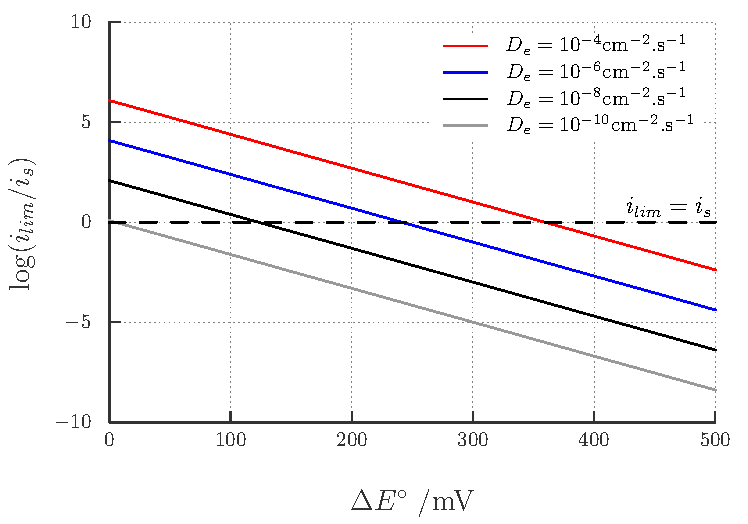
\includegraphics[width=0.87\textwidth]{Graficos/ilimite.pdf}
		        \caption[Dependencia de la mediación redox con $D_e$ y $K$]{Dependecia de la relación $i_{lim}/i{s}$ variando el coeficiente de difusión dentro de la película $D_e$ en función de la separación entre potenciales formales para el mediador y la sonda.}
		        \label{fig:ilimitee}
		      	\end{figure} 

	\subsection{Estabilidad de las películas delgadas mesoporosas de \texorpdfstring{SiO$_2$}{SiO2}}

		Como ya se ha demostrado, al poner en contacto una solución de \ru\space sobre una \pdmF, la película se va cargando con la sonda hasta alcanzar la saturación. Es de esperar que la carga dentro de la película se mantenga constante y que, a partir del voltagrama de máxima adsorción las sucesivas voltametrías sean equivalentes.

		Sin embargo, no es así, y al ciclar constantemente el sistema se obtienen voltagramas como el presentado en la figura \ref{fig:diso_ru1mM}, experimento donde se adsorbió \ru\space \SI{1}{\milli\Molar}. Se observa que la película se va cargando conforme aumenta el número de ciclos, y adsorbe cada más \ru\space hasta llegar a un valor máximo de adsorción, indicado por la curva azul. Si se continúa ciclando el sistema el mismo evoluciona hasta la curva roja, la cual coincide con un voltagrama para \ru\space medido sobre un electrodo de Au desnudo. Esto sugiere que las \pdmF\space se disuelven luego de hacer algunos ciclos de VC.

		Si bien estamos en a un pH ($5.5$) donde la disolución de las \pdmF\space debería ser mínima o nula, las mismas parecen disolverse con bastante facilidad, mostrando siempre el comportamientos del voltagrama de la figura \ref{fig:diso_ru1mM}, independientemente del tratamientos posdepósito o de la concentración de la sonda utilizada. Se diseñaron experimentos para determinar la causa de la disolución, ya que podría ser función del pH, la sonda o el potencial aplicado, entre otras. Se han aislado estas variables dejando sumergidas las \pdmF\space en solución con electrolito soporte (KCl \SI{100}{\milli\Molar}), con y sin \ru\space durante varios días y no se ha observado disolución alguna de las \pdm. Tampoco se ha observado disolución cuando se utilizan sondas neutras o negativas, como \fe, hidroquinona o \fc. En resumen, las \pdmF\space sólo se disuelven cuando se realizan voltametrías consecutivas con solución de \ru\space.
			
		 	\begin{figure}[t!]
				\centering
		 	    \includegraphics[width=0.83\textwidth]{Graficos/Ru1mM-secuencia-continua-hasta-disolucion.pdf}
		        \caption[Disolución de una \pdmF\space en \ru.]{Ciclos sucesivos de VCs para \ru\space \SI{1}{\milli\Molar} en solución de KCl \SI{100}{\milli\Molar}. Se observa aquí como se carga para luego recuperar la señal de un electrodo de Au desnudo, debido a la disolución de la \pdmF.}
		        \label{fig:diso_ru1mM}
		      	\end{figure} 

	    En la figura \ref{fig:ventanas} se graficó la razón entre la intensidad de pico de un electrodo recubierto con \pdmF\space y uno desnudo para tres concentraciones de \ru\space distintas. En estos gráficos se puede fácilmente visualizar la capacidad de preconcentrar y la cantidad de ciclos antes de la disolución. Se pueden dividir en tres zonas, I) zona de carga, II) zona de máxima adsorción y III) zona de disolución o de perdida de la estructura. Todas las medidas que se hicieron en este trabajo fueron realizadas dentro de la zona II, asegurándose la máxima adsorción del \ru\space.


		Al ingresar y adsorberse el \ru\space se produce, por cada ciclo de mediación, una migración de iones y contraiones desde y hacia la película, debido a los cambios de estado de oxidación de la sonda por el potencial aplicado, y a la necesidad de compensar la carga.  Se puede hacer una analogía con los sistemas de rédox poliméricos, en los cuales al colocarlos en una solución con electrolitos se produce un cambio de volumen, denominado \textit{swelling}, debido al ingreso de los mismos\cite{ybarra2005}. En estos sistemas formados por óxidos inorgánicos, mas rígidos, el cambio en el volumen es mínimo,\cite{Malfatti2009} sin embargo la migración de los iones y contraiones parece provocar cambios irreversibles en la estructura de la película mesoporosa que llevan, finalmente, al colapso de la misma.

		 	\begin{figure}[t!]
	 	   	    \begin{subfigure}[t]{0.495\textwidth}
		        	\includegraphics[width=0.95\textwidth]{Graficos/Ru10mM-ventana-preconcentracion.pdf}
		       		\vspace*{-0.3cm}
		       		\caption{$\text{i}_p\mathbin{/}\text{i}_p^{\text{Au}}$ en función del ciclado EQ para \ru\space \SI{10}{\milli\Molar}.}
		         	\label{fig:Ventana_Ru10mM}
		     		\end{subfigure}
	     		\begin{subfigure}[t]{0.495\textwidth}
		        	\includegraphics[width=0.95\textwidth]{Graficos/Ru1mM-secuencia-continua-hasta-disolucion-ventana-trabajo.pdf}
		       		\vspace*{-0.3cm}
		       		\caption{$\text{i}_p\mathbin{/}\text{i}_p^{\text{Au}}$ en función del ciclado EQ para \ru\space \SI{1}{\milli\Molar}.}
		         	\label{fig:Ventana_Ru1mM}
		     		\end{subfigure}
	     		\begin{center}
	     		\begin{subfigure}[t]{0.495\textwidth}
		        	\vspace*{-0.3cm}
		        	\includegraphics[width=0.95\textwidth]{Graficos/Ru0315mM-secuencia-continua-ventana-trabajo.pdf}
		       		\vspace*{-0.3cm}
		       		\caption{$\text{i}_p\mathbin{/}\text{i}_p^{\text{Au}}$ en función del ciclado EQ para \ru\space \SI{0.3}{\milli\Molar}.}
		         	\label{fig:Ventana_Ru0315mM}
		     		\end{subfigure}
		     		\end{center}
	 	   	   	\vspace*{-0.3cm}
	 	   	   	\caption[Intensidad en función del ciclado EQ para \pdmF]{Razón entra la intensidad de pico catódica para \ru\space de un electrodo recubierto con \pdm\space y uno sin recubrir, la línea roja indica cuando $\text{i}_p\mathbin{/}\text{i}_p^{\text{Au}} = 1$. Cabe destacar que al disminuir la concentración de \ru\space en solucón aumenta el poder preconconcentrador. Zona I: adsorción, zona II: máxima preconcentración, zona III: disolución.}
	     		\label{fig:ventanas}
	     	  \end{figure}

	\section{Transporte en \pdm\space mixtas Zr/Si}

			Con la intención de evitar la disolución descrita en la sección anterior y mejorar la resistencia química y mecánica de los sensores, se prepararon películas delgadas silicio incorporando una pequeña cantidad de circonio, las cuales llamaremos \pdmZ. Se conoce que el Zr(IV) es capaz de estabilizar al Si(IV) en medio alcalino\cite{Soler-Illia2004}, de esta forma se espera obtener películas delgadas estables durante las mediciones EQ, sin perder la exclusión de iones ni la la química superficial que ofrece las películas de SiO$_2$. Son muchos los trabajos en la literatura en los cuales depositan películas mesoporosas de ZrO$_2$ puras, mixtas con TiO$_2$, con SiO$_2$, e incluso con VO$_x$ \cite{Soler-Illia2004,Crepaldi2002a,Gimenez2016,Zelcer2013,Calvo20210,Angelome2008}. En este trabajo se utilizó un sol de relación Si/Zr $9\!:\!1$ de forma de evitar la segregación de fases\cite{Soler-Illia2004}. Se estructuraron los poros con Pluronic F127 y se depositaron las películas sobre electrodos de Au y obleas de silicio (consultar sección \ref{sec:soles} para los detalles de la preparación y depósitos del sol). Para la condensación y extracción se eligió el método de alto vacío (en lugar de la clásica calcinación), el cual se desarrolló y se estudiaron los resultados extensamente en este mismo trabajo (ver capítulo \ref{chap:Mesoporosos}).

			En los trabajos de Soler-Illia y col.\cite{Soler-Illia2004} y de Crepaldi y col. \cite{Crepaldi2002a}, los autores concluyen, entre otras cosas, que las \pdmZ\space sufren menor deterioro a los tratamientos térmicos, y sugieren que presentan mejor resistencia a entornos ácidos y básicos respecto de sus homologas, las películas hechas de óxido de silicio exclusivamente. Manzini y col.\cite{Gimenez2016} también reportaron la fuerte resistencia mecánica de las películas de ZrO$_2$ mesoporosas frente a la radiación ionizante.

	 \subsection{Exclusión}

	 	 Al introducir Zr en las películas delgadas se espera un corrimiento del IEP hacia un pH mayor\cite{Kosmulski2014}. Sin embargo al incluir solo un núcleo metálico de Zr cada diez de Si, esperamos mantener un IEP más próximo al del SiO$_2$ y, consecuentemente, observar propiedades similares a las que ya se presentaron para las \pdmF.
	 	 Se evaluó, en primera instancia, si a pH=5,5 las \pdmZ\space presentan capacidad de excluir electrostaticamente sondas negativas. El voltagrama de la figura \ref{fig:fcn-zr} muestra la respuesta del electrodo frente a una solución de \fe\space \SI{1}{\milli\Molar} y se compara con un electrodo de Au desnudo. Claramente se ve que la sonda imposibilitada de ingresar en la película debido a la carga negativa de las paredes de los poros de las \pdmZ. 
				
				\begin{figure}[ht]
				\centering
		 	    \includegraphics[width=0.75\textwidth]{Graficos/Zr-ExclusionFcCN.pdf}
		        \caption[Exclusión electrostática en \pdmZ]{Respuesta comparativa de un electrodo de Au recubierto con \pdmZ\space (sólida) y uno sin recubrir (punteado) frente a una sonda \ferroferri\space \SI{1}{\milli\Molar} en \SI{0.1}{\Molar} de KCl utilizando ECS como referencia.}
		        \label{fig:fcn-zr}
		      	\end{figure} 
	 
	 \subsection{Preconcentración y estabilidad}\label{sub:pcirc}

		 	Para estudiar la capacidad de preconcentrar de las \pdmZ\space se realizaron los mismos experimentos que para las \pdmF. Se puso en contacto un electrodo recubierto con \pdmZ\space con solución de \ru\space de distintas concentraciones. 


	 			\begin{figure}[th]
			   	    \begin{subfigure}[t]{0.325\textwidth}
			        	\includegraphics[width=0.95\textwidth]{Graficos/Zr-Ru1mM.pdf}
			        	\vspace*{-0.40cm}\caption{\aminorutenio\space \SI{1}{\milli\Molar}.}
			         	\label{fig:Zr-Ru1mM}
			     		\end{subfigure}
			   	    \begin{subfigure}[t]{0.325\textwidth}
			        	\includegraphics[width=0.95\textwidth]{Graficos/Zr-Ru01mM.pdf}
			       		\vspace*{-0.40cm}\caption{\aminorutenio\space \SI{0.1}{\milli\Molar}.}
			         	\label{fig:Zr-Ru0.1mM}
			     		\end{subfigure}
		     		\begin{subfigure}[t]{0.325\textwidth}
			        	\includegraphics[width=0.95\textwidth]{Graficos/Zr-Ru001mM.pdf}
			       		\vspace*{-0.40cm}\caption{\aminorutenio\space \SI{0.01}{\milli\Molar}.}
			         	\label{fig:Zr-Ru0.01mM}
			     		\end{subfigure}
			     		\caption[Preconcentración de \aminorutenio\space en \pdmZ]{Adsorción de \ru\space en \pdmZ\space a diferentes concentraciones de la sonda. Los voltagramas grises (\usebox{\gris}) indican el ingreso de la sonda en la red nanoporosa, los negros (\usebox{\negro}) corresponden a la máxima preconcentración y los voltagramas punteados (\usebox{\punteado}) son la respuesta en electrodos de Au desnudo. Todos los voltagramas fueron medidos a \SI{50}{\milli\volt\per\second} en solución de KCl \SI{100}{\milli\Molar}.}
			     		\label{fig:precon_ZR}
		     		\end{figure}
		
		 Como se observa los voltagramas de la figura \ref{fig:precon_ZR}, las \pdmZ, al igual que las \pdmF, adsorben y preconcentran fuertemente una sonda positiva como el \ru,	incluso a concentraciones tan bajas como \SI{10}{\micro\Molar}. Se hicieron ciclos de VCs para evaluar la estabilidad de las \pdmZ\space frente a las mediciones EQ y a la migración de iones que se genera en dicho proceso. 

		 			\begin{figure}[h!]
		 			\vspace*{-6mm}
			   	    \begin{subfigure}[t]{0.495\textwidth}
			        	\includegraphics[width=1\textwidth]{Graficos/Zr-numero-de-ciclo-01mM.pdf}
			        	\vspace*{-10mm}\caption{$\text{i}_p\mathbin{/}\text{i}_p^{\text{Au}}$ en función del ciclado EQ para \ru\space \SI{0.1}{\milli\Molar}}
			         	\end{subfigure}
			     		 \begin{subfigure}[t]{0.495\textwidth}
			        	\includegraphics[width=1\textwidth]{Graficos/Zr-numero-de-ciclo-1mM.pdf}
			        	\vspace*{-10mm}\caption{$\text{i}_p\mathbin{/}\text{i}_p^{\text{Au}}$ en función del ciclado EQ para \ru\space \SI{1}{\milli\Molar}}
			         	\end{subfigure}
			         	\caption[Intensidad en función del ciclado EQ para \pdmZ]{Razón entra la intensidad de pico catódica para \ru\space de un electrodo recubierto con \pdmZ\space y uno sin recubrir, la línea rojo indica cuando la razón = 1. Zona I: zona de carga, zona II: zona de máxima adsorción.}
			         	\label{fig:ventana-zr}
			         	\vspace{3mm}
			     	\end{figure}

		 Se graficó la intensidad de pico relativa a la intensidad en un electrodos de Au desnudo, tal como se hizo para las \pdmF. Aquí se observa que, para \ru\space \SI{0.1}{\milli\Molar} luego de 360 ciclos la intensidad solo disminuyó un 15\%, y, para \ru\space \SI{1}{\milli\Molar} luego de 600 ciclos solo un 20\%  lo que sugiere que la velocidad de disolución es mucho más lenta que para las películas puras de SiO$_2$ (figura \ref{fig:ventana-zr}).
			     		
		 Con el propósito de evaluar la estabilidad de \pdmZ\space con las \pdmF, se han colocado en la figura \ref{fig:zr-comp} dos gráficos. El primero, figura \ref{fig:zr-comp-a}, compara la intensidad relativa a un electrodo de Au en función de la cantidad de ciclos, tanto para \pdmZ\space como para \pdmF. Se verifica en ese mismo gráfico la disolución total de las \pdmF\space luego de unos 100 ciclos, mientras que para las mixtas Zr/Si la señal solo cae un 20\% luego de 600 ciclos. El segundo grafico, figura \ref{fig:zr-comp-b}, muestra las voltametrías cíclicas (para \ru\space sobre \pdmZ) desde el ciclo 180 al 250, donde se puede observar que los voltagramas son prácticamente equivalentes.

		 			\begin{figure}[h!]
		 			\vspace*{-2mm}
			   	    \begin{subfigure}[t]{0.495\textwidth}
			        	\includegraphics[width=1\textwidth]{Graficos/Comparacion-CICLOS-Ru1mM-cal-vac-Zr.pdf}
			        	\caption{Comparación de la razón de la intensidad de pico de \ru\space \SI{1}{\milli\Molar} para Cal\pdmF, Vac\pdmF\space y Vac\pdmZ\space respecto de un electrodo de Au.}
			        	\label{fig:zr-comp-a}
			         	\end{subfigure}
			     		\begin{subfigure}[t]{0.495\textwidth}
			        	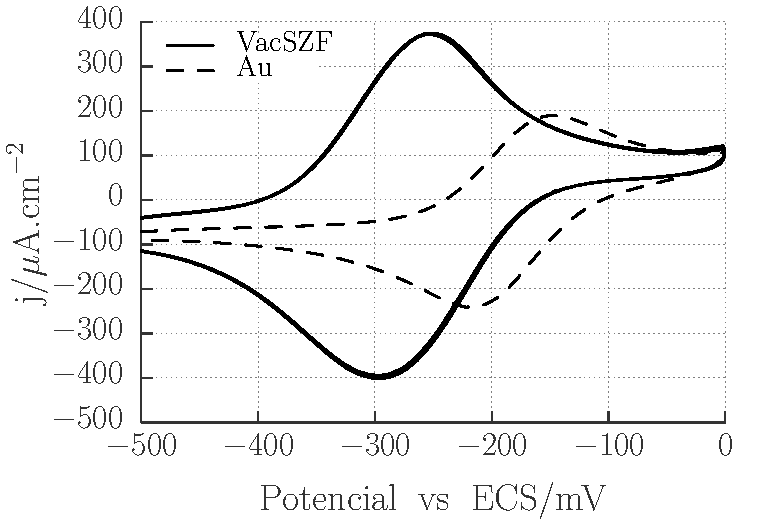
\includegraphics[width=1\textwidth]{Graficos/Zr-Ru1mM-181-246Ciclos.pdf}
			        	\vspace*{-0.40cm}\caption{VCs consecutivas para  \ru\space \SI{1}{\milli\Molar} sobre Vac\pdmZ\space (ciclos 180 al 250) comparado con la respuesta de un electrodo de Au desnudos (punteado).}
			        	\label{fig:zr-comp-b}
			         	\end{subfigure}
			         	\caption[Estabilidad de las \pdmZ]{Estabilidad de las películas \pdmZ\space frente al ciclado electroquímico. (a) Comparación en intensidad con sistemas Cal\pdmF\space y Vac\pdmF. (b) Voltagramas consecutivos correspondientes a los ciclos 180 al 250 donde se observa que todos ellos son prácticamente equivalentes.}
			         	\label{fig:zr-comp}
			     	\end{figure}		

\subsection{Funcionalización}\label{sub_sec_funcionalizaciones_chap_4}

			En esta sección se exponen los resultados obtenidos al incluir y anclar grupos moleculares dentro de los poros. Realizar dichas funcionalizaciones tiene por objetivo de cambiar la naturaleza química superficial de los poros, de forma de modificar las propiedades permeoselectivas de las películas. 

			Para obtener resultados sólidos sobre fenómenos de transporte dentro de las películas es necesario que la estabilidad estructural de las mismas no esté comprometida. 

			En las secciones precedentes se ha demostrado que la incorporación de un 10\% de Zr en la formación de las películas de SiO$_2$ mejora la estabilidad mecánica y la resistencia química sin perder poder de adsorción, incluso frente a \pdmF\space calcinadas. Es por ellos que todos los experimentos que se presentan en esta sección fueron realizados sobre películas mesoporosas de  Si$_{0.9}$Zr$_{0.1}$O$_2$ sintetizadas por el método de alto vacío.

			Las moléculas incorporadas fueron dihexadecilfosfato (DHDP) y 3-amino-\- propil trietoxisilano (APTES). Dicha elección se fundamentó en trabajos previos donde estudian en detalle la incorporación de estás moléculas, ya sea en películas delgadas mesoporosas de SiO$_2$, TiO$_2$, ZrO$_2$ o mixtas.\cite{Calvo2009b,Angelome2008,Fattakhova-Rohlfing2007,Andrieu-brunsen2014,Andrieu-Brunsen2015} Hasta ahora no se han reportado en la literatura trabajos donde se incorporen estas funcionalizaciones sobre electrodos recubiertos con películas delgadas mesoporosas mixtas Zr$_x$Si$_{1-x}$O$_2$. Además, los resultados expuestos en esta sección cuenta con el plus de que fueron obtenidos de un único sensor, es decir, que las reacciones de funcionalización se llevaron en electrodos diferentes de un mismo dispositivo. El capítulo que sigue ahonda en los detalle sobre la fabricación de los sensores.
	
		\subsubsection{Incorporación de DHDP}
	
			La funcionalización con DHDP se llevó a cabo adaptando la reacción utilizada por Angelomé\cite{Angelome2008}. Se utilizó DHDP \SI{3}{\milli\Molar} en películas delgadas de Si$_x$Zr$_{1-x}$O$_2$ (\pdmZ$^P_3$). El detalle de las condiciones experimentales se puede consulta en la sección \ref{sub:funcionalizaci_n_de_las_pdm}, pág. \pageref{sub:funcionalizaci_n_de_las_pdm}. En su trabajo, Angelomé incorpora DHDP en películas mixtas de Si$_x$Zr$_{1-x}$O$_2$ y Si$_x$Ti$_{1-x}$O$_2$. Se concluye allí que la reacción se trata de una unión débil de complejación superficial entre el fosfonato y el centro metálico, en este caso el Zr. El esquema de la figura \ref{esq:dhdp-esquema} representa una \pdmZ$^P_3$ luego de ser funcionalizada.

				 \begin{figure}[ht!]	
					\centering
			 	    \includegraphics[width=\textwidth]{Esquemas/funcionalizaciondhdp.pdf}
			        \caption[Funcionalización con DHDP 3mM]{Esquema donde se representa la reacción de DHDP con \pdmZ\space para obtener películas funcionalizadas con DHDP. Figura adaptada de \textit{Films delgados mesoporosos de óxidos metálicos, mixtos e híbridos. Hacia un diseño racional de nanomateriales funcionales.} Angelomé P., Tesis de Doctorado, Facultad de Ciencias Exactas y Naturales - UBA, 2008.\cite{Angelome2008}}
			        \label{esq:dhdp-esquema}
			      	\end{figure}

			\pagebreak

			Una vez realizada la funcionalización de las películas se llevaron a cabo sobre las mismas mediciones EQ con \fe, \fc\space y \ru. El resultado se presenta en los voltagramas de las figura \ref{fig:dhdp-vc}. 

		    	\begin{figure}[h!]	
					\begin{subfigure}[t]{0.495\textwidth}
			 	    \includegraphics[width=\textwidth]{Graficos/dhdp-FeCN.pdf}
			        \caption{Respuesta utilizando como sonda negativa \ferroferri\space \SI{1}{\milli\Molar}.}
			        \label{fig:dhdp-vc-fe}
			        \end{subfigure}
			         \begin{subfigure}[t]{0.495\textwidth}
			 	    \includegraphics[width=\textwidth]{Graficos/dhdp-FcOH.pdf}
			        \caption{Respuesta utilizando neutra \fc\space \SI{1}{\milli\Molar}.}
			        \label{fig:dhdp-vc-fc}
			        \end{subfigure}
			        \begin{center}
			        \begin{subfigure}[t]{0.60\textwidth}
			 	    \includegraphics[width=\textwidth]{Graficos/dhdp-Ru.pdf}
			        \caption{Respuesta utilizando positiva \aminorutenio\space \SI{1}{\milli\Molar}.}
			        \label{fig:dhdp-vc-ru}
			        \end{subfigure}
			        \end{center}
			        \caption[Voltagramas de \pdmZ$^P_3$ con \aminorutenio, \fc\space y \ferroferri]{Respuesta comparativa entre \pdmZ\space funcionalizadas con DHDP y sin funcionalizar. Para cada experimento se tomaron 90 voltagramas consecutivos en KCl \SI{100}{\milli\Molar} a \SI{50}{\milli\volt\per\second}.}
			        \label{fig:dhdp-vc}
			      	\end{figure}

		    En los caso del \fe\space y el \fc\space (gráficos \ref{fig:dhdp-vc-fe} y \ref{fig:dhdp-vc-fc} respectivamente) se observa un leve aumento de la densidad de corriente en las películas funcionalizadas con DHDP respecto de las no funcionalizadas. Sin embargo, la señal, a igualdad de condiciones, sigue siendo muy pequeña comparada con un electrodo de Au desnudo (j$^p_{FeCN}\!=$\SI{340}{\micro\ampere\per\square\cm} y j$^p_{FcOH}\!=$\SI{98}{\micro\ampere\per\square\cm}). Esto indica que el comportamiento es similar en ambos casos: el \fe\space queda prácticamente excluido y el \fc\space permea en mayor o menos medida.

		   % En el caso del \fe\space se observa que  la sonda negativa sigue estando fuertemente excluida de las películas, tanto estén o no funcionalizada con DHDP (figura \ref{fig:dhdp-vc-fe}). El incremento que se observa en la densidad de corriente en las \pdmZ$^P_3$, posiblemente debido a una leve permeación, sigue siendo extremadamente pequeño cuando se lo compara con un electrodo de Au desnudo (j$^p_a=$\SI{340}{\micro\ampere\per\square\cm}), indicando que el DHDP no compensa la carga negativa de las películas y continúan repeliendo electrostáticamente la sonda negativa. En ambos experimentos, sobre \pdmZ\space y , se tomaron 90 voltagramas consecutivos, donde la respuesta electroquímica permanece prácticamente invariante para cada experimento.
 
		    %Para el caso del \fc\space también se observa un leve incremento de la señal cuando las \pdmZ\space se funcionalizan con DHDP. La incorporación del DHDP parece de alguna forma agilizar el proceso de difusión de la sonda neutra hacia la superficie del eletrodo (figura \ref{fig:dhdp-vc-fc}.

		    En la figura \ref{fig:dhdp-vc-ru} se compara la respuesta electroquímica luego de 90 ciclos para \pdmZ\space y \pdmZ$^P_3$\space para \ru\space \SI{1}{\milli\Molar}. Como ya se mencionó anteriormente en la sección \ref{sub:pcirc}, pág. \pageref{sub:pcirc}, la sonda positiva se adsorbe paulatinamente en las \pdmZ\space hasta llegar a la saturación. En las películas funcionalizadas con DHDP no pasa lo mismo. Se observa que desde el primer ciclo la señal del \ru\space corresponde a la de una especie libre, no adsorbida. A medida que aumenta el número de ciclos electroquímicos la sonda ingresa en el mesoporoso rápidamente, llegando a saturación a partir del ciclo 10 aproximadamente (figura \ref{fig:dhdp-vc-ru}). En contrapartida en el caso de las \pdmZ\space requiere mas de 50 ciclos llegar a la saturación. Es interesante destacar que la capacidad final de adsorción no cambia entre los sistemas con o sin DHDP. Esto hecho sugiere que a medida que el \ru\space se adsorbe desplaza al fosfonato para mantener constante la concentración de \ru\space dentro de los poros.

		    Los resultados de incorporar DHDP en los poros parece no tener efecto sobre la carga de las películas, ya que no se ven alteradas cualitativamente las propiedades de transporte. Sigue preconcentrando \ru, excluyendo \fe\space y permitiendo la percolación de \fc. Sin embargo se observa que se agiliza el transporte de las sondas hacia el electrodo. Esto se pone de minifiesto ya que en las películas \pdmZ$^P_3$, para \ru,  desde los primero ya se observa la respuesta como una sonda libre en solución, para luego evolucionar como una sonda adsorbida en una cantidad de ciclos mucho menos que en las \pdmZ. Más adelante una vez analizados los resultados de funcionalizar películas con APTES se hace una discusión más amplia sobre estas observaciones.
			
			%Otro fenómeno, que posiblemente afecte el trasporte, es la capa hidrofóbica que se forma dentro de los poros, debida a las largas cadenas de hidrocarburos del DHDP. Dicha capa dificulta la adsorción de \ru\space dentro de \pdmZ$^P_3$ a la vez que favorece la libre difusión del \ru\space hacia el electrodo. 

		\subsubsection{Incorporación de APTES}
			
			La incorporación del 3-aminopropil trietoxisilano se hizo en base al protocolo utilizado por Calvo\cite{Calvo20210}. En dicho trabajo se estudió profundamente la adición de esta molécula en películas delgadas mesoporosas de SiO$_2$, TiO$_2$ y mixtas. La autora concluye que la incorporación de APTES modifica el estado de carga superficial de las \pdm\space lo cuál, a un pH determinado, altera sensiblemente el transporte de sondas electroquímicas cargadas. Se ejemplifica en el esquema de la figura \ref{esq:aptes-esquema} la funcionalización con APTES incorporada en \pdmZ\space y su equilibrio ácido-base.

				 \begin{figure}[ht!]	
					\centering
			 	    \includegraphics[width=\textwidth]{Esquemas/funcionalizacionaptes.pdf}
			        \caption[Funcionalización con APTES 1mM]{Esquema donde se representa la reacción de APTES con \pdmZ\space para obtener películas funcionalizadas con grupos aminos y la dependencia de la carga con el pH. Figura adaptada de \textit{Films delgados mesoporosos híbridos conteniendo el grupo amino: una plataforma para el diseño y producción de membranas permeoselectivas}, Calvo A., Tesis de Doctorado, Instituto de investigación e ingeniería ambiental - UNSAM, 2010.\cite{Calvo20210}}
			        \label{esq:aptes-esquema}
			      	\end{figure}

			\vspace*{3mm}Se funcionalizaron \pdmZ\space con APTES \SI{1}{\milli\Molar} y \SI{10}{\milli\Molar} (\pdmZ$^N_{1}$ y \pdmZ$^N_{10}$ respectivamente) con el objetivo de obtener diferentes grados de funcionzalición\cite{Calvo20210,Angelome2008,Fuertes2010}. Al igual que en el caso en que se funcionalizó con DHDP, se exponen en la figura \ref{fig:aptes1mM-vc}, los voltagramas obtenidos al utilizar \fe, \fc\space y \ru\space como sondas.

			Para la respuesta con \fe\space (figuras \ref{fig:aptes1mM-vc-fe}) se puede observar un pico correspondiente a la adsorción de de la sonda, sin embargo al ser el pico tan pequeño se puede concluir que las películas siguen excluyendo fuertemente la sonda de carga negativa.

			En los casos que se usó \fc\space (figura \ref{fig:aptes1mM-vc-fc}) se observa que la corriente de pico es similar para ambos, \pdmZ\space y \pdmZ$^N_1$. Sin embargo, se observa un cambio cualitativo en la respuesta de la sonda: la diferencia de potenciales de pico catódico y anódico se encuentran desplazados en las \pdmZ$^N_1$ respecto de las \pdmZ. Por otra parte la diferencia entre los potenciales de pico catódico y anódico es menos de \SI{60}{\milli\volt}, indicando que la especie se encuentra adsorbida. 

				 \begin{figure}[ht!]	
					\begin{subfigure}[t]{0.495\textwidth}
			 	    \includegraphics[width=\textwidth]{Graficos/aptesfecn-1mM.pdf}
			        \caption{Respuesta utilizando como sonda negativa \ferroferri\space \SI{1}{\milli\Molar}.}
			        \label{fig:aptes1mM-vc-fe}
			        \end{subfigure}
			        \begin{subfigure}[t]{0.495\textwidth}
			 	    \includegraphics[width=\textwidth]{Graficos/aptesfeoh-1mM.pdf}
			        \caption{Respuesta utilizando como sonda neutra \fc\space \SI{1}{\milli\Molar}.}
			        \label{fig:aptes1mM-vc-fc}
			        \end{subfigure}
			        \begin{center}
			        \begin{subfigure}[t]{0.60\textwidth}
			 	    \includegraphics[width=\textwidth]{Graficos/aptesru-1mM.pdf}
			        \caption{Respuesta utilizando como sonda positiva \aminorutenio\space \SI{1}{\milli\Molar}.}
			        \label{fig:aptes1mM-vc-ru}
			        \end{subfigure}
			        \end{center}
			        \caption[Voltagramas de \pdmZ$^P_3$ con \aminorutenio\space y \ferroferri]{Respuesta comparativa entre \pdmZ\space funcionalizadas con APTES \SI{1}{\milli\Molar} y sin funcionalizar. Para cada experimento se tomaron más de 90 voltagramas consecutivos en KCl \SI{100}{\milli\Molar} a \SI{50}{\milli\volt\per\second}.}
			        \label{fig:aptes1mM-vc}
			      	\end{figure}

		  
		  En la figura \ref{fig:aptes1mM-vc} se exponen los resultados de comparar la respuesta de \ru\space en \pdmZ\space y en \pdmZ$^N_1$. Allí se ponen de manifiesto dos cambios en los voltagramas correspondientes a las películas funcionalizadas y a las que no fueron funcionalizadas: el primero es la disminución de la corriente de saturación y el segundo es la cantidad de ciclos necesarios para llegar a dicha saturación. Los resultados sugieren que los grupos NH$_3^+$ parecen neutralizan parte de la carga negativa de las películas, dificultando la adsorción del \ru\space (la incorporación es mucho más lenta y solo luego de 100 ciclos alcanza la saturación) y disminuyendo la capacidad de adsorción de las \pdmZ$^N_{1}$ para esta sonda, reduciendola aproximadamente a la mitad que en películas no funcionalizadas. 

		  Se obtuvieron resultados equivalentes para las tres sondas al funcionalizar las \pdmZ\space con APTES \SI{10}{\milli\Molar} (figura \ref{fig:aptes10mM-vc}). Esto sugiere que se alcanzó el grado máximo de funcionzalización de las \pdmZ\space con una solución de APTES \SI{1}{\milli\Molar}.

	 	\subsubsection{Discusión sobre las funcionalizaciones}

	 	 En los apartados anteriores quedó demostrado que al funcionalizar las \pdmZ\space se afecta significativamente la permeoselectividad y los propiedades de transporte de las \pdm. Aquí se busca resumir y analizar en modo sintético los datos expuestos anteriormente. 

	 	 En el gráfico de la figura \ref{fig:pot-int} se expone la evolución de los ciclos electroquímicos para \ru\space en distintos sistemas. Para ello se extrajeron los valores de máxima intensidad de pico anódico en función del potencial al aparece en dicho máximo. Los resultados de dicho grafico fueron medidos en un sensor con distintos electrodos: de Au sin recubrimiento, recubierto con \pdmZ\space sin funcionalizar, recubierto con \pdmZ\space funcionalizado con APTES (\pdmZ$^N_1$) y recubierto con \pdmZ\space funcionalizado con DHDP (\pdmZ$^P_3$).

	 			 \begin{figure}[h!]	
					\centering
			 	    \includegraphics[width=0.90\textwidth]{Graficos/pot-int.pdf}
			        \caption[Evolución de la señal de \ru\space para distintos sistemas]{Intensidad de corriente de pico anódico vs potencial de pico de \aminorutenio\space para diferentes funcionalizaciones sobre películas delgadas mesoporosas de Si$_{0.9}$Zr$_{0.1}$O$_2$. Los puntos rojos correponden a la señal de un electrodo de Au desnudo.}
			        \label{fig:pot-int}
			        \vspace*{3mm}
			      	\end{figure}

	 	 En el gráfico se puede analizar como evoluciona la adsorción de \ru\space \SI{1}{\milli\Molar} en distintos sistemas. Para facilita la interpretación se remarcó el potencial correspondiente a \ru\space libre en solución ($E^p_{sol}$), el potencial para \ru\space adsorbido ($E^p_{ads}$) y la densidad de corriente de \ru\space obtenida en un electrodo de Au desnudo ($j^p_{Au}$). En ese mismo electrodo (Au desnudo) la respuesta es, obviamente, invariable de ciclo a ciclo, salvo por la dispersión propia de cualquier medida EQ. La densidad de corriente relativa a este electrodo indica la capacidad para preconcentrar de cada sistemas, mientras mayor sea la diferencia, mayor será la capacidad de preconcentrar.

	  	 El potencial de pico anódico (ubicado en el eje de las abscisas) indica la evolución de la especie \ru\space libre a la especie \ru\space adsorbido. Se pueden extraer algunas observaciones interesante para cada uno de los sistema: \pdmZ, \pdmZ$^P_3$ y \pdmZ$^N_1$. En las películas sin funcionalizar el sistema evoluciona con un régimen mixto (caracterizado por escalada suave de corriente en función del potencial), en el cuál se manifiesta el transporte de carga mediante \ru\space adsorbido y el transporte de masa mediante \ru\space libre, el cuál difunde dentro de los poros como un especie en solución. Para el caso de películas funcionalizadas con DHDP se observa que se encuentra muy favorecida la difusión de \ru\space al electrodo y que rápidamente el sistema evoluciona al adsorbido, manteniendo la misma capacidad de preconcentrar la sonda. Finalmente en el caso en que se funcionalizaron las \pdmZ\space con APTES se observa que el \ru\space está impedido de difundir y que la corriente aumenta de forma abrupta cerca del potencial que corresponden con la especia \ru\space adsorbida. Este fenómeno se puede apreciar bien en los voltagramas de la figura \ref{fig:compaptesnoaptes} en la cuál se comparan los primeros 14 ciclos sobre una \pdmZ\space sin funcionalizar con los primeros 45 ciclos en una película funcionalizada con APTES. Se destaca en la figura con flechas la evolución en cada sistema, en particular en las películas funcionalizadas se ve como la corriente aumenta pero el potencial correpondiente siempre al la de la especie adsorbida.

	 	 		 \begin{figure}[h!]	
					\centering
			 	    \includegraphics[width=0.80\textwidth]{Graficos/comparacionszfszfn.pdf}
			        \caption[Evolución de la señal de \ru\space para distintos sistemas]{Voltagramas de \ru\space sobre películas funcionalizadas con APTES (\pdmZ$^N_1$) y sin funcionalizar (\pdmZ) donde se destaca la diferente cinética de adsorción para cada sistema.}
			        \vspace*{4mm}
			        \label{fig:compaptesnoaptes}
			      	\end{figure}


	 	 Por otra parte en las \pdmZ$^N_1$ la densidad de corriente de pico la mitad que en una \pdmZ, indicando que la capacidad de preconcentración disminuyó con un factor aproximado de $1/2$. Ambas observaciones, tanto el impedimento de libre difusión del \ru\space cómo la disminución en la capacidad de preconcentrar se pueden atribuir al cambio de carga superficial en las \pdmZ\space debido a la incorporación de los grupos amino, que al pH de trabajo se encuentran protonados como NH$_3^+$.

	 	 			

	 	  %Cabe destacar la rápida evolución en los sistemas con DHDP (respecto de los no funcionalizados) debido a la hidrofobicidad, lo cual favorece la difusión del \ru\space hacia el electrodo (\ru\space libre). En el sistema con APTES la adsorción respecto de los otros sistemas (\pdmZ$^P_3$\space y \pdmZ) es lenta y disminuye sensiblemente la capacidad preconcentradora de la sonda.

\section{Conclusiones parciales}
	
	Durante los capítulos previos se han estudiado y desarrollado métodos para depositar películas delgadas mesoporosa de SiO$_2$ y Si$_{0.9}$Zr$_{0.1}$O$_2$  sobre electrodos de Au. A su vez se idearon mecanismos de condensación y extracción del surfactante a temperaturas por debajo de los \SI{130}{\celsius}. 

	Una vez terminadas estas etapas, se realizó un exhaustivo estudio de las diferentes respuestas electroquímica en función de las interacciones de las \pdm\space con las sondas utilizadas. Se verificó la exclusión del \ferroferri\space (negativa), la permeación del \fc\space (neutra) y la adsorción del \aminorutenio\space (positiva). Los resultados sobre estas últimas permitieron por primera vez, obtener la concentración de \ru\space dentro de las películas, evaluar la capacidad de preconcentración, estimar la constante de Langmuir y calcular valores de coeficientes de difusión, ya sea por transferencia de masa (como en el caso del \fc) o por transferencia de carga vía \textit{electron hopping}, como en el caso del \ru.

	Se simularon voltametrías cíclicas por elementos finitos para interpretar resultados de un experimentos de mediación rédox, donde se intentó mediar la respuesta electroquímica de una sonda a través de una \pdm\space saturada con \ru. Se establecieron las condiciones de contorno para las cuales se podría dar o no dicho proceso y, avanzando con las simulaciones, se pudo determinar si el fenómeno dominante es el de mediación o el de permeación. Se realizó un análisis más profundo donde se establecieron cuales son los procesos que podrían tener lugar dentro de las películas porosas, y como influye sobre estos el coeficiente de difusión dentro de la película ($D_e$ y la constante de equilibrio entre la sonda en solución y el mediador $K$.

	Se demostró la disolución por completo de las \pdmF\space durante el ciclado electroquímico. Este comportamiento se ha verificado para cualquier tipo de película de SiO$_2$ (ya sea calcinada o no, sobre ITO o sobre Au). En la mayoría de los casos la disolución es completa a partir de ciclo número 100. Este fenómeno se ha interpretado como una disolución catalizada por el ciclado electroquímico debida a la migración de iones y contraiones entre la película y la solución. Con el objetivo de minimizar dicha disolución, se sintetizaron películas delgadas mesoporosas mixtas Si\textbar Zr con el método de alto vacío (desarrollado en este mismo trabajo). Se verificaron las mismas capacidades selectivas (exclusión, permeación y preconcentración) que las películas de SiO$_2$, pero con una resistencia química y mecánica muy superior, pudiéndose llevar a cabo hasta 600 ciclos electroquímicos con una disminución de la señal sólo del 20\%.

	Una vez superados los problemas de estabilidad de las \pdm\space sometidas al ciclado electroquímico, se avanzó en la selectividad de las películas. Se trabajó exclusivamente con películas Si$_{0.9}$Zr$_{0.1}$O$_2$ obtenidas por el método de alto vacío. Sobre estos sistemas se llevaron a cabo funcionalizaciones con el objetivo de modificar las propiedades de transporte. Se incorporó individualmente en dos electrodos distintos de un mismo sensor, dihexadecilfosfato y 3-aminopropil trietoxisilano. El analisis de los resultados de las mediciones electroquímicas mostraron que las propiedades de transporte se vieron modificadas significativamente debido a estas funcionalizaciones. Se estudió como se modfica la cinética de adsorción del \aminorutenio\space al incorporar los distintos tipos de moléculas. Los resultados obtenidos en función de dichas modificaciones químicas se utilizarán en el próximo capítulo para llevar a cabo pruebas de concepto para el desarrollo de sensores EQ multipropósito.



%---------------------------------------------------------------------------------------------------------

%HACE FALTA LA CARACTERIZACION COMPLETA DEL MESO SIZR????  y Colocarlo en el capitulo 4???	
%FTIR - SEM - EPA - CA - EDS???? OPTICO

